% Intended LaTeX compiler: pdflatex
\documentclass[a4paper,12pt]{article}
                              \usepackage[utf8]{inputenc}
                              \usepackage{sectsty}
                              \sectionfont{\normalfont\scshape}
                              \subsectionfont{\normalfont\itshape}
                              \usepackage[round,authoryear]{natbib}
                              \usepackage{amsmath}
                              \newtheorem{theorem}{Theorem}
                              \newtheorem{assumption}{Assumption}
                              \newtheorem{acknowledgement}{Acknowledgement}
                              \newtheorem{algorithm}{Algorithm}
                              \newtheorem{axiom}{Axiom}
                              \newtheorem{case}{Case}
                              \newtheorem{claim}{Claim}
                              \newtheorem{conclusion}{Conclusion}
                              \newtheorem{condition}{Condition}
                              \newtheorem{conjecture}{Conjecture}
                              \newtheorem{corollary}{Corollary}
                              \newtheorem{criterion}{Criterion}
                              \newtheorem{definition}{Definition}
                              \newtheorem{example}{Example}
                              \newtheorem{exercise}{Exercise}
                              \newtheorem{lemma}{Lemma}
                              \newtheorem{notation}{Notation}
                              \newtheorem{observation}{Observation}
                              \newtheorem{problem}{Problem}
                              \newtheorem{proposition}{Proposition}
                              \newtheorem{remark}{Remark}
                              \newtheorem{result}{Result}
                              \newtheorem{summary}{Summary}
                              \newtheorem{Hypothesis}{Hypothesis}
                              \newcommand{\qed}{\hspace*{\fill} {\em Q.E.D.}}
                              \usepackage{pdftexcmds}
                              \usepackage{minted}
                              \usepackage{textcomp}
                              \usepackage{hyperref}
                              \usepackage{graphicx}
                              \usepackage{mathtools}
                              \mathtoolsset{showonlyrefs=true}
                              \linespread{1.3}
                              \usepackage[right=3cm, left=3cm,top=3cm,bottom=3cm]{geometry}
                                          \makeatletter
\newcommand{\citeprocitem}[2]{\hyper@linkstart{cite}{citeproc_bib_item_#1}#2\hyper@linkend}
\makeatother
\usepackage[round,authoryear]{natbib}
\setcitestyle{authoryear, round, comma, aysep={;}, yysep={,}, notesep={, }}
\author{Jan Boone\thanks{Tilburg University, Department of Economics, Tilec and CEPR, E-mail: \textit{j.boone@uvt.nl}.}}
\date{\today}
\title{Pricing above value: selling \emph{to} an adverse selection market}
\hypersetup{
 pdfauthor={Jan Boone\thanks{Tilburg University, Department of Economics, Tilec and CEPR, E-mail: \textit{j.boone@uvt.nl}.}},
 pdftitle={Pricing above value: selling \emph{to} an adverse selection market},
 pdfkeywords={},
 pdfsubject={},
 pdfcreator={Emacs 29.0.50 (Org mode 9.5.4)}, 
 pdflang={English}}
\begin{document}

\maketitle
\maketitle
\begin{abstract}
This paper shows that selection incentives in downstream markets distort upstream prices. It is possible for inputs to be priced above the value that the good has for final consumers. We apply this framework to pharmaceutical companies selling drugs to a health insurance market with adverse selection problems. We specify the conditions under which drugs are sold at prices exceeding treatment value. Another feature of the model is an excessive private incentive to reduce market size, e.g. in the form of personalized medicine.
\end{abstract}

\textbf{Keywords:} adverse selection, pricing above value, vertical relations, pharmaceutical prices

\textbf{JEL codes:} I13, I11


\newpage

\section{Introduction}
\label{sec:orge276c13}

Consider a value chain where firms in an upstream market \(U\) sell inputs to firms in a downstream market \(D\) and the latter sell to final consumers. When considering the input prices set by firms in \(U\), there are a number of common sense results: 1. do not set the input price above the final consumers' valuation of your input; 2. try to innovate to make your product attractive to a bigger group of final consumers and 3. reduce your price as the downstream market becomes more competitive.

However, when \(U\) sells to a market \(D\) with adverse selection problems, these three results do not necessarily hold. If low types in \(D\) mimic the high types, it is optimal for \(U\) to set prices above final consumers' valuation of the input. Limiting the types of final consumers that value your product raises profits. And input prices increase with the competition intensity in downstream market segments.

An interesting market to apply this framework to is the health insurance market (\(D\)) where pharmaceutical companies in market \(U\) sell drugs to insurers to be included in their insurance contracts. Health insurance markets are known for their adverse selection problems and almost daily there are stories in the news about pharmaceutical companies charging "outrageous" prices for their treatments.\footnote{Examples include \url{https://nyti.ms/2NvLoZx}, \url{https://nyti.ms/2bHXkFj} and \url{https://nyti.ms/2nKMJ2a}.} Although it is hard to put a value on an additional year of life to see whether prices are above treatment value, for anticancer drugs "in 1995 patients and their insurers paid \$54,100 for a year of life. A decade later, 2005, they paid \$139,100 for the same benefit. By 2013, they were paying \$207,000" (\citeprocitem{23}{Howard et al. 2015, 149}). Most regulators in the world use less than \$200k as the monetary value of a life year and indeed at the World Oncology Forum the "prevailing opinion was that \ldots{} the cost of the new generation of drugs is getting out of all proportion to the added benefit" (\citeprocitem{5}{Cavalli 2013}).

It has been noted that "prices of \ldots{} drugs in the so-called 'specialty' pharmaceutical market have been increasing over time" (\citeprocitem{23}{Howard et al. 2015, 140}). The promise of specialty or precision medicine was "to give 'the right drug to the right patient' to maximize the effectiveness and safety of the treatment" (\citeprocitem{15}{Garattini, Curto, and Freemantle 2015}). However, up till now this targeting of treatments has not lived up to this promise and one reason is that these treatments turn out to be extremely expensive. It is not clear that we can afford precision medicine. To illustrate, in oncology there are treatments costing \$300,000 while they "only result in minimal benefit" (\citeprocitem{10}{Doble 2016}).

We propose a set-up with upstream pharmaceutical companies selling drugs to downstream insurers for inclusion in their health insurance contracts. The health insurance market suffers from adverse selection. The condition we need for our results is that low risk types are tempted to buy the insurance contract aimed at high risk types. Below we cite evidence supporting that this is the relevant case in health insurance markets. In this case, pharmaceutical firms can charge prices in excess of their treatments' value for patients and still have their treatments covered by insurance. To reduce low risk rents insurers distort the high type's allocation upwards by covering a treatment that is expensive. Any change that makes the high risk type contract more attractive to the low type makes covering this treatment more attractive and increases the excess profits that upstream firms can earn. We denote these excess profits --i.e. profits in excess of treatment value-- supra profits.

We show that supra profits are increasing in the competitiveness of the high type market: as the high type market becomes more competitive, the insurance premium tends to fall making the high contract more attractive to the low type. Further, targeting of pharmaceutical R\&D investments on subgroups (precision medicine) tends to increase supra profits. We derive conditions under which such targeting of R\&D is privately profitable and socially wasteful. The last result sheds light on developments in specialty drugs or personalized medicine where higher prices are easier to spot than improved treatments. Finally, the introduction of generic drugs helps to increase prices of patented drugs. To the extent that people can decide to go without insurance, the insurance premium cannot exceed the total value of the insurance contract. Generic drug competition leads to prices below the value of treatment thereby creating the "space" for patented drugs to charge prices above value.

The main assumption we need is that low types want to buy the generous high type contract. We provide two rationales for this assumption. First, in the main model the high risk type market segment is more competitive than the low type segment in the insurance market. In our health insurance context this implies that high risk individuals are more sensitive to value differences between insurance contracts than low risk types. There is empirical evidence showing this is the relevant case. First, the insurance premium elasticity is substantially higher for employees with a chronic condition (high risk) than without (\citeprocitem{36}{Parente, Feldman, and Christianson 2004}). One explanation for this is that high risk types are more likely to have experience with healthcare and therefore know more about quality differences between treatments. As they are better informed, they are more sensitive to quality differences between plans (\citeprocitem{17}{Gaynor, Ho, and Town 2015}). A second intuition is that high risk types tend to have lower incomes and therefore pay more attention to value differences between plans.\footnote{The correlation between health status and income is well documented in the empirical health literature (\citeprocitem{14}{Frijters, Haisken-DeNew, and Shields 2005}; \citeprocitem{13}{Finkelstein and McGarry 2006}; \citeprocitem{18}{Gravelle and Sutton 2009}; \citeprocitem{34}{Munkin and Trivedi 2010}). Potential explanations for this correlation include the following. High income people are better educated and hence know the importance of healthy food, exercise etc. Healthy food options tend to be more expensive and therefore better affordable to high income people. Or (with causality running in the other direction) healthy people are more productive and therefore earn higher incomes.} Hence, consumers' insurer switching probability falls with income. Also, people on low income are more price sensitive when choosing health insurance. In the same vein, the higher educated and the wealthier are less price sensitive (\citeprocitem{22}{Ho, Hogan, and Scott Morton 2017}; \citeprocitem{1}{Atherly, Dowd, and Feldman 2004}; \citeprocitem{2}{Auerbach and Ohri 2006}; \citeprocitem{39}{Saltzman 2019}; \citeprocitem{38}{Royalty and Solomon 1999}).\footnote{There are also papers suggesting that people with lower health status tend to be less price elastic when choosing insurance. These papers tend to be based on age as an indicator of health status: older people tend to have lower health status (\citeprocitem{43}{Strombom, Buchmueller, and Feldstein 2002}; \citeprocitem{38}{Royalty and Solomon 1999}). Others find no difference in elasticity between age groups (\citeprocitem{8}{Costa and Garcia 2003}). One reason for the seemingly lower price elasticity is that older people (people with low health status in general) tend to be better informed about the quality of the different health plans and the treatments they cover. This can explain why they react less to price changes and to plan quality information published by the government or an employer (\citeprocitem{3}{Beaulieu 2002}).}

Next to differences in competitiveness, a second rationale why low risk types mimic high risk types is a lack of information/rationality. Low risk types buy the contract with low out-of-pocket expenditures (targeted at high risk types) because they (incorrectly) believe this contract to be more generous than it actually is, e.g. because they believe it covers more treatments and a wider network of providers (\citeprocitem{20}{Handel and Kolstad 2015}). It has also been documented in the Dutch health insurance market that low risk types tend to buy the low deductible contract that is optimal for high risk types (\citeprocitem{19}{Handel et al. 2020}). Hence, empirically, there are reasons to believe that low risk types tend to mimic high risk types as we assume in this paper.

Our analysis is related to the following strands of literature. There are a number of explanations for high drug prices found in the literature (\citeprocitem{23}{Howard et al. 2015}). However,  these cannot fully explain why prices would exceed treatment value. To illustrate, an explanation that is often mentioned is that with health insurance people want a treatment, no matter what the cost since the insurer pays (most of) the price. This is true ex post: once I have insurance, the effects of the cost of treatment are reduced for me. Economists tend to refer to this as moral hazard. However, why would I buy insurance coverage for a treatment that costs more than the benefit it provides? Dropping such a treatment from the contract leads to a bigger reduction in the premium than the loss in expected utility. Hence, an insurer --whether or not it has market power-- benefits from removing such treatments from its insurance contract. This threat of not being covered by an insurance contract limits the price a pharmaceutical company can ask for patented drugs.

Similarly, high sunk costs of R\&D are often mentioned to explain high treatment prices (\citeprocitem{16}{Garrison and Towse 2017}). Although high fixed/sunk costs can explain high prices in competitive markets (by limiting entry), this mechanism is not obvious for a monopoly market where a firm is protected by a patent. Since a monopolist tries to appropriate most or all of the surplus from its customers, its sunk fixed costs are not directly relevant for setting prices. And also here, if the treatment is too expensive, it should be dropped by the insurer from the contract.\footnote{In free market systems, the insurer can decide what to cover or not in its contracts. In regulated market systems, like the Netherlands, the government often prescribes which conditions need to be covered by basic insurance but does not define which treatments need to be covered.}

When comparing drug prices between countries, a number of institutional features are often mentioned. One is whether the health insurance market is run by the government or via a market with private insurers. To illustrate, in public healthcare systems politicians tend to find it hard to refuse reimbursement of a treatment on the basis of its price; this creates upward pressure on prices.\footnote{Note that citizens may actually agree with politicians' point of view here (\citeprocitem{29}{McCabe, Claxton, and Tsuchiya 2005}).} A classic example is the coverage of proton beam therapy in the NHS before any cost-benefit analysis was done: "proton beam therapy has not been the subject of a technology appraisal by the National Institute for Health and Clinical Excellence" and at the time there was no "reliable, objective evidence that proton beam treatment improved clinical outcomes" (\citeprocitem{21}{Hawkes 2012}). Economists have compared proton beam therapy to the death star (\citeprocitem{27}{Langreth 2012}). Other explanations for cross country price differences include GDP per head (richer countries tend to pay more), whether the drug prices are bargained over centrally or by insurers individually, country regulations regarding reference pricing etc. (\citeprocitem{9}{Danzon and Taylor 2010}).

What we add to this literature is that the extent of selection problems in the health insurance market affects drug prices. To the best of our knowledge there is no direct evidence on this relation. However, we do know that the US tends to pay far more for patented drugs than other countries and that price differences between European countries are relatively small (\citeprocitem{33}{Mulcahy et al. 2021}; \citeprocitem{45}{Young et al. 2017}). Adverse selection problems are bigger in the US (with many people going without insurance) than in Europe where all countries have relatively high insurance coverage (often mandatory or automatic insurance) and in this sense reduced selection problems.

Other papers focus on the relation between prices and disease rarity: the lower the prevalence of a disease, the higher the prices for drugs treating it. In the context of orphan drugs, this is sometimes referred to as payers valuing rarity (\citeprocitem{30}{Medic et al. 2017}; \citeprocitem{31}{Messori, Cicchetti, and Patregani 2010}). If the insurance premium is determined by the budget constraint of the marginal insured, an inverse relation exists between disease prevalence and drug price (\citeprocitem{25}{Kamphorst and Karamychev 2021}). We offer a complementary explanation for this inverse relation via the selection incentives on the health insurance market.

In terms of the mechanism design literature, our focus on a binding incentive compatibility constraint for low types is in line with the countervailing incentives literature (\citeprocitem{28}{Lewis and Sappington 1989}). This literature considers type dependent outside options, which we generate through differing demand elasticities for different types. Although we use health insurance and adverse selection to illustrate our model, the mechanism applies in any screening model where the incentive compatibility constraint is binding for the low type.

Our paper is organized as follows. First, we illustrate our main effect in an insurer duopoly model. Then we present our general framework to show that supra profits appear when low risk types in the health insurance market tend to mimic the high types. We derive conditions under which private incentives for developing specialty drugs are excessive from a social point of view. We discuss the effects of bounded rationality and conclude with a discussion of policy implications.

\section{Duopoly example}
\label{sec:example}
\label{sec:example}

To see how it is possible that an insurer pays more for a treatment than the treatment's value to the insured, consider the following example with two treatments and two competing insurers. The example introduces the notation and illustrates the mechanics of the result.

Denote the two treatments 1 and 2; both treatments are produced at marginal costs normalized to zero: \(c_1 = c_2 =0\). Treatment 1 is under patent. Treatment 2 is off patent and sold by competing generic drug producers at a price equal to marginal costs. The values of these treatments are given by \(v_1,v_2\) resp. and are the same for each patient. Value \(v_i\) captures things like life years gained, improvement in quality of life, increased productivity etc. (\citeprocitem{16}{Garrison and Towse 2017}). Although it is not straightforward to measure this in practice, conceptually the value of a treatment is well defined. We aim to show that pharmaceutical companies can profitably charge a price in excess of this value and still be covered by insurance plans.

The competing insurers \(a,b\) sell insurance to a customer who can be either of risk type \(l\) (probability \(\phi\)) or type \(h\) (probability \(1-\phi\)). Type \(k=l,h\) needs treatments 1,2 with probability \(\psi_{1k},\psi_{2k}\). We assume single crossing: \(\psi_{ih} \geq \psi_{il}\) for \(i=1,2\) and to simplify notation in this example assume that \(\psi_{2h} = \psi_{2l} = \psi_2\). Hence, the high risk consumer has a strictly higher probability of needing treatment 1: \(\psi_{1h}>\psi_{1l}\). Thus the insurer's expected costs are higher for type \(h\) than for type \(l\) as \(h\) is more likely to need treatment.

We assume that the consumer buys insurance to get access to treatments. That is, without insurance, the consumer goes without treatment.\footnote{To simplify notation, we normalized \(c_1=c_2=0\). For the access to care interpretation, think of \(c_1,c_2\) being high enough that a patient without insurance cannot afford them even at cost price.} It is well documented that people without health insurance tend to forgo treatment as they have difficulty financing it. These access issues have been stressed both in the popular press (\citeprocitem{7}{Cohn 2007}) and in academic journals (\citeprocitem{35}{Nyman 1999}; \citeprocitem{40}{Schoen et al. 2008}; \citeprocitem{41}{Schoen et al. 2010}). Many governments are concerned about health consumption inequality caused by income differences and design policies to make healthcare accessible to low income families (\citeprocitem{42}{Schokkaert and van de Voorde 2011}).

Each insurer offers two contracts (which can be identical in case of a pooling outcome), each contract aimed at a consumer type. We write the value/utility of the contract for type \(k=1,2\) as follows:
\begin{equation}
\label{eq:5}
u_{k} = \alpha \psi_{1k} x_{1k} v_1 + \psi_{2} x_{2k} v_2 - \sigma_k
\end{equation}
where \(x_{ik} \in [0,1]\) denotes the probability that treatment \(i\) is covered by contract \(k\) (below we have that \(x_{ik}\) equals either 0 or 1) and \(\sigma_k\) denotes the price/premium of contract \(k\). Value \(v_i\) denotes the utility of receiving the treatment in case the consumer needs it (with probability \(\psi_{ik}\)) compared to not receiving this treatment. Note that falling ill in itself can cause a disutility for the individual. Taking this into account would add a constant to the expression in \eqref{eq:5} which we leave out to ease notation.

The use of \(\alpha \in [0,1]\) is a "technical trick". Strictly speaking, it denotes the probability that treatment 1 is available to the insurer.\footnote{In this sense, \(x_{ik}\) denotes the probability that i is covered conditional on it being available to the insurer.} We think of \(\alpha\) as being equal to one throughout the paper; but can deduce the value of treatment 1 for the insurer by considering the effect on the insurer's profits of a small decrease in \(\alpha\).\footnote{This gives us the convenience of differentiating instead of taking the discrete difference between profits with (\(\alpha=1\)) and without (\(\alpha=0\)) treatment 1 being covered.} In particular, to understand how \(p_1 > v_1\) is possible, we will derive conditions under which the insurer's profits are \emph{strictly} increasing in \(\alpha\) \emph{even if} \(p_1 = v_1\).

The incentive compatibility (IC) constraints for these contracts can be written as follows.
\begin{align}
\label{eq:2}
u_h &\geq  \alpha \psi_{1h} x_{1l} v_1 + \psi_{2} x_{2l} v_2 - \sigma_{l} \\
\label{eq:4}
u_l &\geq   \alpha \psi_{1l} x_{1h} v_1 + \psi_{2} x_{2h} v_2 - \sigma_h
\end{align}
The first equation, \(IC_h\), implies that the high type is better off choosing the high contract (yielding utility \(u_h\)) than to buy the low type's contract (which yields her utility equal to the right hand side of \eqref{eq:2}). To illustrate, the \(h\) type needs treatment 1 with probability \(\psi_{1h}\), but the \(l\) contract provides this treatment with probability \(x_{1l}\) (assuming \(\alpha=1\)) in which case she gets utility \(v_{1}\); the price of this contract equals \(\sigma_{l}\). And, similarly, \(IC_l\) implies that the low type is better off buying the \(l\) contract --yielding \(u_l\) -- than buying the \(h\) contract which yields her utility equal to the right hand side of \eqref{eq:4}. These constraints capture intra-brand competition faced by the insurer: if the \(h\) contract becomes too attractive, \(l\) types buy this contract instead of the \(l\) contract (\eqref{eq:4} is violated).

As we will see below, pricing a treatment above its value is possible if the \(h\) market is more elastic than the \(l\) market. To illustrate how elasticities are determined we introduce income and competition intensities in the model.

A simple way to introduce income effects is as follows. If insurance contract \(k\) from insurer \(a\) gives utility \(u_k^a\), then an insured's overall utility is given by
\begin{equation}
\label{eq:50}
(y_k+u_k^a)^{\eta}
\end{equation}
with income \(y_k \ge 0 \text{ and } \eta \in \langle 0,1]\). There are two insurers competing on a Hotelling beach of length 1 with consumers distributed uniformly (with density 1) along the beach. Insurer \(a\) is on the left hand side of the beach and insurer \(b\) on the right hand side. A fraction \(\phi\) of consumers (on each location) is type \(l\) and a fraction \(1-\phi\) is \(h\). The travel cost over the Hotelling beach for type \(k\) is denoted by \(t_k, k=l,h\). If insurer \(a\) offers utility \(u_k^a\) and insurer \(b\) offers \(u_k^b\), then \(a\)'s market share \(q_k\) is given by the indifferent consumer at position \(q_k \in [0,1]\) on the \(k\) market:
\begin{equation}
\label{eq:18}
(y_k+u_k^a)^{\eta} - t_k q_k = (y_k+u_k^b)^{\eta} - t_k (1-q_k)
\end{equation}
For the indifferent consumer the utility buying from \(a\) minus the travel cost to \(a\) equals the utility from \(b\) minus the travel cost to \(b\). Hence, \(a\)'s market share can be written as
\begin{equation}
\label{eq:19}
q_k = \frac{1}{2} + \frac{(y_k+u_k^a)^{\eta} - (y_k+u_k^b)^{\eta}}{2t_k}
\end{equation}
Then we can define type \(k\)'s demand elasticity as
\begin{equation}
\label{eq:51}
\varepsilon_k = \left| \frac{\partial q_k}{\partial \sigma_k^a} \frac{\sigma_k^a}{q_k} \right| = \frac{\eta}{t_k}\frac{\sigma_k}{(y_k+u_k)^{1-\eta}}
\end{equation}
in symmetric equilibrium with \(u_k^a=u_k^b=u_k,\sigma_k^a=\sigma_k^{b}=\sigma_k\).

Before interpreting these results, let us briefly motivate the functional forms used. The Hotelling model of competition is fairly standard (\citeprocitem{44}{Tirole 1988}). It allows us to model competition with inelastic market demand but elastic demand for the firm. The inelastic demand is useful here for two reasons. First, it is easy to combine with IC constraints for the two customer types. Second, it is straightforward to compare the value of the treatment \(v_i\) with the price of the treatment \(p_i\) charged by the manufacturer. If consumers have differing values for \(v_i\) (elastic demand), it is not clear to which value \(v_i\) the price \(p_i\) should be compared to claim that pricing is excessive (the average \(v_{i}\), the median or maximum \(v_i\)?). With this set-up we can transparently make the claim that pricing is excessive in the sense that the price exceeds the treatment's value for each customer.

If both insurers offer the same utility level, \(a\)'s market share equals \(1/2\). If \(u^a_k > u^b_k\), \(a\) is relatively more attractive and its market share exceeds \(1/2\). The pace at which \(a\)'s market share increases with the difference between \(u_k^a\) and \(u_k^b\) is determined by travel cost \(t_k\) and parameter \(\eta\). The lower \(t_k\), the more market share responds to utility differences offered by insurers and the more competitive the market is.

The parametrization in equation \eqref{eq:50} is chosen for similar reasons as the Hotelling model. Because \(u_k^a\) enters linearly in this expression, we can use the standard IC constraints and compare \(v_i\) to the price \(p_i\) that the manufacturer charges. We interpret \(y_k\) as type \(k\)'s income that is spent on other goods and services. It acts to make overall utility less elastic as income increases in case \(\eta<1\). Someone with a low income is more sensitive to changes in, say, the insurance premium than someone with a high income (\citeprocitem{22}{Ho, Hogan, and Scott Morton 2017}).

Summarizing equation \eqref{eq:51}, \(k\)'s demand elasticity decreases with \(t_k\): the more competitive the Hotelling market (lower \(t_k\)), the more elastic is type \(k\)'s demand for insurer \(a\)'s contract. Lower income \(y_k\) also leads to more elastic demand in case \(\eta<1\).

We finish the section with an example where indeed \(IC_l\) is binding. As the goal is to show that something is \emph{possible} we simplify by assuming \(\eta=1,y_k=0\) for \(k=l,h\). We first assume that \(IC_h\) is slack (and check later that this assumption is correct; see the proof of lemma \ref{Hotelling_equilibrium}).

The profit insurer \(a\) makes on type \(k\) buying its contract is given by \(\sigma_k^{a} - \alpha\psi_{1k}x_{1k}p_1 - \psi_{2k}x_{2k}p_2\): premium minus expected costs for type \(k\) where insurers' costs are determined by the prices \(p_{i}\) charged by the research labs. Solving equation \eqref{eq:5} for \(\sigma_{k}\) and substituting this into the expression for the per type profit gives:
\begin{equation}
\label{eq:6}
\pi_k^a = \alpha\psi_{1k}x_{1k}(v_1-p_1)+\psi_{2k}x_{2k}(v_2-p_2)-u_k
\end{equation}
and the insurer's overall profits are given by
\begin{equation}
\label{eq:7}
\Pi^a = \phi q_l^a \pi_l^{a} +(1-\phi)q_h^a\pi_h^{a}
\end{equation}
Fraction \(\phi\) of low types times insured \(a\)'s market share on the \(l\) market times \(a\)'s per customer profit on the \(l\) market; and similarly for the \(h\) market segment.

With \(p_1=v_1\) and \(p_2=0\) due to competition on the generic (off-patent) market, we write insurer \(a\)'s optimization problem as:
\begin{align}
\nonumber
    \max_{u_l^a,u_h^a,x_{1h}^a,x_{2l}^a,x_{2h}^a} & \phi \left(\frac{1}{2} + \frac{u_l^a-u_l^b}{2t_l} \right) (\psi_2 x_{2l}^a v_2 -u_l^a) \\
    \label{eq:20}
     & + (1-\phi) \left(\frac{1}{2} + \frac{u_h^a-u_h^b}{2t_h} \right) (\psi_2 x_{2h}^a v_2 -u_h^a) \\ \nonumber
     & + \lambda_l (u_l^a - u_h^a + \alpha v_1 x_{1h}^a (\psi_{1h}-\psi_{1l}))
\end{align}
where \(\lambda_l\) denotes the Lagrange multiplier on \(IC_l\) constraint \eqref{eq:4}.

In the appendix, we derive the following equilibrium outcome.
\begin{lemma}
\label{Hotelling_equilibrium}
In the Hotelling model, assume that \(p_1 =v_1\) and \(t_l - t_h > v_1 (\psi_{1h}-\psi_{1l})\). Then in equilibrium, it is the case that \(x_{1h}=x_{2h}=x_{2l}=1\), \(x_{1l} \in [0,1]\) and
\begin{align}
\label{eq:21c}
\lambda_{l} &= \frac{1}{2} \frac{t_l-t_h-\alpha v_1 (\psi_{1h}-\psi_{1l})}{\frac{t_h}{1-\phi}+\frac{t_l}{\phi}} > 0 \\
\label{eq:21d}
\left. \frac{d\Pi}{d\alpha}\right|_{p_1=v_1} &= (\psi_{1h}-\psi_{1l}) v_1 \lambda_l > 0
\end{align}
\end{lemma}

The assumption in the lemma is that the \(h\) market is (sufficiently) more competitive than the \(l\) market (\(t_h < t_l\)). Under this assumption an equilibrium exists where \(IC_l\) is binding.\footnote{Note that our focus on a binding \(IC_l\) implies that we do not need to introduce co-payments which help separate types when \(IC_h\) is binding (\citeprocitem{37}{Rothschild and Stiglitz 1976}).} The shadow price \(\lambda_l\) of the (\(IC_l\)) constraint is positive under the assumptions that we made: the \(l\) type wants to mimic the \(h\) type who gets a relatively better deal as the \(h\) market is more competitive than the \(l\) market.

Equation \eqref{eq:21d} implies that even if \(p_1=v_1\), the insurer's profits are strictly increasing in \(\alpha\). Hence, the producer of treatment 1 can ask more than \(p_1 = v_1\) --the final consumers' valuation of the treatment-- and the insurer will still cover this treatment in its health insurance contract. If \(p_1 = v_1\) would be the maximum price firm \(1\) can charge for its treatment, insurer \(a\) would be indifferent between covering the treatment or not: \(d\Pi^{a}/d\alpha = 0\) at \(p_1 = v_1\). As this derivative is strictly positive, the lab can charge more than \(p_1=v_1\). For our purposes here, there is no need to characterize the solution further.

The reason why the insurer is willing to cover a treatment which is sold at a price in excess of its value to patients is that covering the treatment helps to increase the \(l\) type's premium \(\sigma_{l}\). In other words, the treatment has value for the insurer in addition to the utility created by the treatment for the insured. The insurer's \(h\) contract competes with its own \(l\) contract. The more attractive the \(h\) contract becomes, the lower \(\sigma_{l}\) has to be; this intra-brand competition is captured by \(IC_{l}\). Covering the expensive treatment relaxes the \(IC_l\) constraint and the value of relaxing \(IC_l\) is given by its shadow price \(\lambda_l > 0\). Since the \(h\) type is more likely to need the treatment than the \(l\) type, covering the treatment makes the \(h\) contract less attractive to the \(l\) type. This allows the insurer to increase \(\sigma_l\) and profits.

Note the role of generic drugs, here captured by treatment 2, being sold at a price below their value (\(p_2 < v_2\)). As these drugs are patent-free, any company can produce them thereby competing the price down below value. Here we assume that the price is competed down to marginal costs (normalized to 0) on the generic drugs market. But all we need, is that \(p_2 < v_2\) on the generic market to make \(p_1>v_1\) possible. Generic drugs are needed for our argument to "create space" for patented firms to charge prices above their treatments' values. To see this, consider the case where \(p_2=v_2\). Together with \(p_1>v_1\) this makes a contract covering treatment 1 loss-making because a consumer is not willing to pay more than \(\psi_{1k} v_1 + \psi_{2k} v_2\) for an insurance contract covering both treatments. Hence in this case, treatment 1 with \(p_1>v_1\) will be dropped by the insurer.

We show in the appendix (Lemma \ref{Hotelling_lambda}) that \(\lambda_l\) is increasing in \(t_l\) and decreasing in \(t_h\). In words, as competition in the \(h\) market makes the \(h\) contract more attractive for the \(l\) type, \(IC_l\) becomes "more binding" and treatment 1 more valuable to insurers. This allows lab \(i\) to increase its price \(p_i\).


\begin{figure}[htbp]
\centering
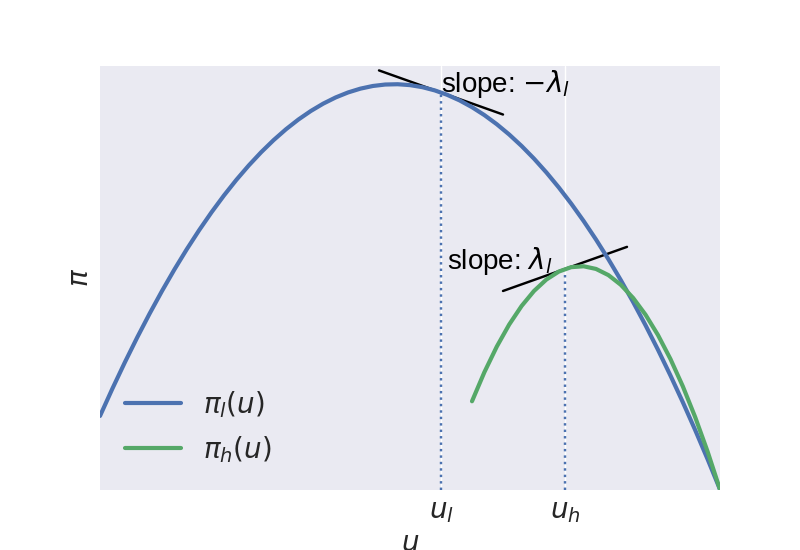
\includegraphics[width=.9\linewidth]{profitfunctions.png}
\caption{\label{fig:profitfunctions}Insurer \(a\)'s profits \(\pi(u^a,\theta_l),\pi(u^a,\theta_h)\) as a function of \(u^a\).}
\end{figure}

Figure \ref{fig:profitfunctions} illustrates the lemma above.\footnote{This figure is based on parameter values: \(\phi=0.5,v_1(\psi_{1h}-\psi_{1l})=1,\psi_2v_2=5,t_h=1,t_l=3,\eta =1,y_l=y_h=0\).} As can be seen in the figure, the \(l\) market is more profitable than the \(h\) market in that profits on the \(l\) market exceed \(h\) profits over the relevant range of \(u\). This is intuitive since \(l\) customers are cheaper in expectation than \(h\) types. In addition, for the insurer to attract customers on the \(h\) market, a larger utility level needs to be left to its customers than on the \(l\) market. This can be due to the fact that \(h\) customers have more experience with treatments and are better able to compare the values offered by different insurance plans. Or \(h\) types (high risk/low health status) tend to have low income and hence pay a relatively low premium \(\sigma_h\) leading to high \(u_h\). Hence, the profit maximizing level of \(u_h\) exceeds that of \(u_l\). But the utility left to \(h\) customers cannot be too high, because this would induce \(l\) customers to buy the \(h\) contract.\footnote{If the \(h\) market would become too small, an insurer can decide to stop serving this market segment. We assume throughout the paper that the \(h\) market is big enough that the insurer keeps on selling to \(h\) types.} The distance \(u_h - u_l\) in the figure is determined by \(IC_l\) holding with equality.\footnote{In the figure, \(u_l\) denotes the symmetric equilibrium outcome on the \(l\) market and \(u_h\) on the \(h\) market. The former is chosen higher than its profit maximizing level --\(u_{l}\) is to the right of the \(u^a\) value maximizing \(\pi_{l}\) -- and the latter lower, if one would consider each market in isolation. At the margin, the loss in profits of not being able to lower \(u_l\) equals the loss of not being able to increase \(u_h\) (which equals \(\lambda_{l}\)).}


\section{Framework}
\label{sec:org62fbe65}

In this section we generalize the framework above. Let \(P\) denote the set of treatments that are currently under patent and \(O\) the set of treatments where the patent has run out ("open" as in open source). To simplify the exposition we assume that \(\psi_{il}<\psi_{ih}\) for each \(i \in P\). For \(j \in O\) we assume \(\psi_{jl} \leq \psi_{jh}\). This ensures that single crossing is satisfied in our set up.\footnote{See Boone and Schottmüller \citeprocitem{4}{2017} for an analysis of the health insurance market where single crossing is violated.}

Insurers \(\iota \in \{a,b,c,...,n\}\) offer contracts \(((x_{il}^{\iota},x_{jl}^{\iota},\sigma_l^{\iota})_{i \in P, j \in O},(x_{ih}^{\iota},x_{jh}^{\iota},\sigma_h^{\iota})_{i \in P, j \in O})\), where the first contract is intended for type \(l\) and the second for \(h\). A contract specifies the probability \(x_{ik} \in [0,1]\) that a treatment is covered and a premium \(\sigma_k\) for \(k=l,h\).

Then the utility for type \(k=l,h\) of buying the contract meant for \(k\) is given by
\begin{equation}
\label{eq:11}
u_k = \sum_{i \in P} \alpha_i \psi_{ik} x_{ik} v_i + \sum_{j \in O} \psi_{jk} x_{jk} v_j - \sigma_k
\end{equation}
where we drop the insurer \(\iota\) superscript to ease notation. Utility consists of the probability that consumer \(k\) needs the treatment \(\psi_{ik} [\psi_{jk}]\) multiplied by the probability that the treatment is covered by the contract \(\alpha_i x_{ik} [x_{jk}]\) times the value of the treatment \(v_i [v_j]\) minus the premium \(\sigma_k\). As above, \(\alpha_i \in [0,1]\) is a technical convenience to determine the value of treatment \(i\) for the insurer. The assumption is that the agent cannot afford the treatments without insurance and hence \(v\) denotes the value of the treatment compared to the best affordable (i.e. without insurance) alternative treatment.

The incentive compatibility constraints can be written as
\begin{align}
\label{eq:12} \tag{$IC_l$}
u_l &\geq  u_h - \sum_{i \in P} \alpha_i x_{ih} v_i (\psi_{ih}-\psi_{il}) - \sum_{j \in O} x_{jh} v_j (\psi_{jh}-\psi_{jl})  \\
\label{eq:12a} \tag{$IC_h$}
u_h &\geq  u_l + \sum_{i \in P} \alpha_i x_{il} v_i (\psi_{ih}-\psi_{il}) + \sum_{j \in O} x_{jl} v_j (\psi_{jh}-\psi_{jl})
\end{align}
Type \(l\) prefers to buy the \(l\) contract which gives utility \(u_l\) rather than buy the \(h\) contract which gives utility equal to the right hand side of \eqref{eq:12}. Similarly for type \(h\). These are the same constraints as \eqref{eq:2} and \eqref{eq:4} but written in a way to stress the importance of \(\Delta \psi_i = \psi_{ih}-\psi_{il}\): the difference in falling ill for the \(h\) and \(l\) types. We denote the Lagrange multiplier on constraint \((IC_k)\) by \(\lambda_k\).

We assume that treatments in the set \(O\) are sold by competing generic drug producers under Bertrand competition with price equal to marginal costs, which we normalize to zero: \(p_j = c_j =0\) for \(j \in O\). The marginal cost of contract \(k\) for the insurer is given by the expected costs of the contract where costs are determined by treatment prices.
\begin{equation}
\label{eq:14}
c_k = \sum_{i \in P} \alpha_i \psi_{ik} x_{ik} p_i
\end{equation}
As the price of \(j \in O\) treatments is normalized to 0, the expected cost of type \(k\) is given by the sum over all patented treatments \(i \in P\) of the probability that \(k\) will receive treatment times the price \(p_i\) of treatment.

The appendix derives the following properties of the solution.
\begin{lemma}
\label{Baseline_results}
Assume \(p_i = v_i\) and \(\alpha_i \in \langle 0,1]\) for \(i \in P\), then we have that \(\lambda_{l}>0\) implies that \(\lambda_h=0\), \(x_{ih}=x_{jh}=x_{jl}=1\) and \(x_{il} \in [0,1]\); further, \(p_i >v_i\) implies \(x_{il} =0\).
\end{lemma}

With \(p_i \leq v_i\), both contracts can cover all treatments. But \(p_i > v_i\) implies that the low type's contract does not cover treatment \(i\). For the low type the treatment price cannot exceed value. Intuitively, \(l\) consumers do not want to pay more for treatment \(i\) than it is worth. And \(x_{il}\) does not help the insurer to reduce intra-brand competition because type \(h\) does not want to buy the \(l\) contract. But \(x_{ih}=1\) is possible in case \(p_i > v_i\). Further, if \(IC_{l}\) is binding (\(\lambda_{l} > 0\)), then \(IC_{h}\) is not (\(\lambda_{h} =0\)). In words, it cannot be the case that \(l\) types would like to buy the \(h\) contract while at the same time \(h\) would like to buy the \(l\) contract.

\section{Supra profits}
\label{sec:org7d0b066}

We consider two contractual arrangements that lead to a profit for the patent holder that exceeds the value of its innovation; we call these extra rents "supra profits". First, we consider the innovator using a two-part tariff which captures most non-linear pricing schemes like quantity discounts (lower price per unit if you buy more). Then we consider the case where the innovator can only use a linear fee (a fixed price per unit).

\subsection{two-part tariff}
\label{sec:orgd3682ff}

The easiest way to see the main effects of this paper is to assume that innovators sell treatments to insurers using two-part tariffs. It turns out that the intuitions we find here, carry over to the case of linear pricing.

To characterize the optimal prices set by innovator \(i\), we first derive the insurers' equilibrium response to the linear part \(p_i\) of the tariff. The insurers set a premium \(\sigma\) which can be different for the \(h\) and \(l\) markets. As above, we define the elasticity of the \(k\) type with respect to the premium \(\sigma_k\) as \(\varepsilon_k = |\frac{\partial q_k}{\partial \sigma_k} \frac{\sigma_k}{q_{k}}|\) and assume that \(\varepsilon_h > \varepsilon_l\).

The following assumption ensures that we are in the relevant parameter space that allows for supra profits. First, equation \eqref{eq:33} implies that \(\lambda_l >0\) (see Lemma \ref{Two_part_tariff} in the appendix). Further, for the insurers' optimization problem to be well defined, we need that the "average elasticity" on the two markets exceeds 1.\footnote{If the average elasticity is below 1, it is optimal for the insurer to set the premium at \(+\infty\). Discarding this possibility is without loss of generality.} Throughout this paper, we assume that both conditions are satisfied.

\begin{assumption}
\label{Elasticities}
\begin{align}
\label{eq:33}
c_h \varepsilon_h (1- \varepsilon_l )-c_l \varepsilon_l(1-\varepsilon_h) > 0 \\
\label{eq:33a}
\phi \varepsilon_l + (1-\phi) \varepsilon_h > 1
\end{align}
\end{assumption}

Lemma \ref{IC_l_binding} in the appendix shows that \eqref{eq:33} can be written as a comparison of elasticity and cost differences. \((IC_{l})\) is binding if the elasticity difference is big compared to the cost difference. Intuitively, if the cost difference is too big, the \(h\) contract will be too expensive to be attractive for the \(l\) type and \(IC_l\) is not binding. If the cost difference is small, the higher elasticity on the \(h\) market reduces the mark-up on the \(h\) contract compared to the \(l\) contract to such an extent that the \(h\) contract is attractive to the \(l\) type: \(IC_l\) is binding. As mentioned in the Introduction, low risk types tend to buy high risk contracts, making binding \(IC_l\) the relevant case in health insurance markets. 

The following lemma derives properties of insurance markets and treatments that tend to lead to high supra profits. With two-part tariffs, the linear tariff is set equal to treatment value, \(p_i=v_i\). The fixed fee is then used to appropriate the supra profits. As in equation \eqref{eq:21d}, \(\lambda_l>0\) implies that even with \(p_i=v_i\), insurers are willing to pay an additional fixed fee to cover treatment \(i\).

\begin{lemma}
\label{Comparative_static_lambda}
Supra profits are proportional to \(\tau_i = \lambda_l v_i \Delta \psi_i\) where \(\Delta \psi_{i} = \psi_{ih} - \psi_{il}\). Further, the shadow price \(\lambda_l\) on the low type's IC constraint is:
\begin{itemize}
\item increasing in \(\varepsilon_h\) and decreasing in \(\varepsilon_l\),
\item decreasing in \(c_h\) and increasing in \(c_l\).
\end{itemize}

Relative to other patented treatments in \(P\), the supra profit of treatment \(i\) increases in \(\Delta \psi_i\).
\end{lemma}

As in the Hotelling model, we find that supra profits \(\tau_i\) are increasing in \(\lambda_l\). Hence, we find that supra profits are increasing in the difference between \(\varepsilon_h\) and \(\varepsilon_l\). The more competitive the \(h\) market becomes, compared to the \(l\) market, the lower the mark-up on the \(h\) contract compared to the \(l\) contract. This makes the \(h\) market more attractive to the \(l\) type and hence the latter's IC constraint "more binding". Similarly, as the difference \(c_h-c_l\) falls, the \(h\) market becomes more attractive for insurers to compete on which, in turn, makes the \(h\) contract more attractive to \(l\) types.

When explaining differences in pharmaceutical prices between countries, attention is focused on institutional features like income per head, who bargains with pharmaceutical companies (e.g. government vs. individual insurers), use of reference pricing and cost effectiveness analysis (\citeprocitem{32}{Morton and Kyle 2011} and references therein). Lemma \ref{Comparative_static_lambda} suggests that selection incentives on the health insurance market can play a role as well. As an illustration of this point, selection problems in US health insurance tend to be seen as worse than in European countries with competitive health insurance markets (like the Czech Republic, Germany, Israel, the Netherlands). The latter countries have automatic/mandatory coverage levels above 90\% of the population in contrast to the US where a large share of the population goes without health insurance.\footnote{Consider the first two rows of the OECD Health Systems Characteristics Survey (\url{https://qdd.oecd.org/data/HSC}) showing the share of the population obtaining basic primary health care coverage through automatic or compulsory insurance coverage. For all European countries this is above 90\% and for most 99\% or 100\%. For the US this is less than one third.} Also branded drug prices in the US are far higher than in Europe (\citeprocitem{33}{Mulcahy et al. 2021}). The analysis here suggests that these two phenomena are connected.

Another factor determining treatment prices is the (individual rationality) constraint that consumers are willing to buy insurance in the first place. If drug prices increase to such an extent that \(u_k < 0\) in equation \eqref{eq:11}, consumers stop buying health insurance because the expected benefit is lower than the price (premium). The introduction of generic drugs in the past decades which --due to competition-- are priced below value (\(p_j < v_j\)) creates the space for patented drugs to price above value and still the value of insurance is bigger than or equal to \(\sigma\). Generic drug prices are lower in the US than in Europe which allows branded drug producers to charge higher prices before the individual rationality constraint is binding (\citeprocitem{33}{Mulcahy et al. 2021}).

The first two comparative statics in the lemma compare the effects of different health insurance systems, e.g. differences between countries. Next, we compare --within a system-- which treatments claim the highest supra profits. We do this as follows. Consider two treatments, 1 and 2; which treatment captures a higher supra profit compared to the value it offers? Using the expression for \(\tau_{i}\) in the lemma:
\begin{equation}
\label{eq:42}
\frac{\tau_1/v_1}{\tau_2/v_2} = \frac{\Delta \psi_1}{\Delta \psi_2}
\end{equation}
Hence drugs with a clear distinction between high risk likely users and low risk occasional users (high \(\Delta \psi_i\)) tend to earn high supra profits. One can think of two reasons why \(\Delta \psi_i\) is high for a treatment \(i\): the first is exogenous to the R\&D lab and the second endogenous. First, it can be a matter of biology: some people suffer from diabetes and others do not. The difference between the prevalence of diabetes among high and low risk types determines \(\Delta \psi_i\) and firm \(i\) cannot change this.\footnote{Note the following distinction: type 2 diabetes tends to be endogenous to an individual's lifestyle but exogenous to an R\&D lab. Here we focus on the exogeneity with respect to the lab.}

Second, R\&D lab \(i\) can invest in projects that are targeted at sub-populations of patients with a disease. This captures the "transition away from the production of 'one-size-fits-all' treatments towards targeted treatments" (\citeprocitem{11}{Dugger, Platt, and Goldstein 2018}). With precision or personalized medicine, the treatment takes the patient's underlying mechanism of the disease into account. Such targeted therapies require the co-development of diagnostic tools to identify the optimal treatment for individual patients. Biomarkers are used to define the subset of patients who benefit from the treatment. The use of biomarkers in clinical trials has increased substantially over time (\citeprocitem{6}{Chandra, Garthwaite, and Stern 2018}). According to our model this goes hand-in-hand with an increase in the number of drugs with high supra profits.

Advantages of precision medicine include faster development and smaller/cheaper trials because the drugs are targeted at smaller groups (\citeprocitem{6}{Chandra, Garthwaite, and Stern 2018}). Better clinical results for the sub-population of patients targeted by the treatment. Ideally, lower healthcare expenditure because of the cheaper development and the fact that the drugs are used for smaller groups. However, the last effect has not materialized as personalized medicine turns out to be very expensive.

What are the ways and incentives for research labs to focus on precision medicine? Pharmaceutical companies need to select the most promising among the drug targets identified in early stages of research to pursue further (\citeprocitem{12}{Emmerich et al. 2021}; \citeprocitem{26}{Knowles and Gromo 2003}). There are two margins along which they can decide to focus on targeted drugs. The extensive margin where they prioritize targeted projects above more generic projects. The intensive margin where they decide to narrow down a given project by investing in the discovery of (more) biomarkers. This decision is partly informed by science but it turns out that there is an important role for marketing and financial directors (\citeprocitem{26}{Knowles and Gromo 2003}).

Although biomarkers "divide the market of treatable patients into groups and clusters, thus reducing market share" (\citeprocitem{24}{Jakka and Rossbach 2013}), this targeting can be profitable in its own right beyond the (socially) beneficial effects mentioned above. In particular, we show that this partitioning of the market is profitable even if no extra social value is created by targeting the treatment. In this sense, there is an excessive incentive for pharmaceutical companies to target treatments with precision medicine.

To capture this idea of excessive targeting, we introduce a parameter \(\zeta\) with the properties that \(d\psi_{ih}/d\zeta <0\) and \(d\Delta \psi_i/d\zeta>0\). This we call "high type targeting". In words, innovator \(i\) focuses on a high type targeting strategy (lab \(i\) increases \(\zeta_i\)) if its treatment will be effective for only a subset of high types (\(d\psi_{ih}/d\zeta_i <0\)) but for an even smaller set of low types (\(d\Delta\psi_i/d\zeta_i>0\)). To illustrate, consider a disease with different strains. Focusing treatment \(i\) on a particular strain that is more prevalent under high than low types, leads to a fall in \(i\)'s market share under \(h\) types --as not all \(h\) types have this strain-- and to an even bigger fall in market share under \(l\) types as they are even less likely to feature this strain.

The lemma shows that a treatment which is more high type targeted leads to higher supra profits. This does not imply that targeting is necessarily a profitable strategy as it shrinks the market for the treatment. We come back to this below.

To the extent that the specialty pharmaceutical market and  personalized medicine are examples of high type targeting, the result implies that they have contributed to the rise in treatment prices documented in the Introduction. This is also our explanation for the observation that "payers value rarity": prices tend to be high for (orphan) drugs with very small patient populations. If such drugs are hardly used by high types (low \(\psi_{ih}\)) and even fewer low types (high \(\Delta \psi_i\)) prices and supra profits will be high.

\subsection{linear pricing and separation}
\label{sec:org394eb30}

Consider the case where the innovating firm cannot use a two-part tariff but only linear pricing (a fixed price per unit). To capture the supra profits, firm \(i\) cannot use the fixed fee (of the two-part tariff) but has to set \(p_i > v_i\). We know from lemma \ref{Baseline_results} that \(p_i>v_i\) implies \(x_{il}=0\): the insurer drops treatment \(i\) in the \(l\) contract. Hence, firm \(i\) weighs a higher price \(p_i\) against a smaller group of customers using the treatment.

The following proposition presents the condition under which setting \(p_i>v_i\) maximizes \(i\)'s profits and we derive the comparative static results with respect to the supra profits.
\begin{proposition}
\label{Linear_price_above_value}
If \(\psi_{il} \leq \Delta \psi_i (1-\varepsilon_l (1-\frac{c_l}{\sigma}))\) then the profit maximizing \(p_{i}\) satisfies
\begin{equation}
\label{eq:56}
\frac{p_i-v_i}{v_i} = \frac{\phi}{(1-\phi)\psi_{ih}} \Delta \psi_i (1-\varepsilon_l (1-\frac{c_l}{\sigma})) > 0
\end{equation}
where the premium for the \(l\) type, \(\sigma\), is defined by equation \eqref{eq:37} in the appendix.

The supra profit \(\frac{p_i-v_i}{v_i}>0\) is
\begin{itemize}
\item increasing in \(\varepsilon_h\) and decreasing in \(\varepsilon_l\);
\item decreasing in \(c_h\) and increasing in \(c_l\);
\item increasing in high type targeting \(\zeta_i\).
\end{itemize}
\end{proposition}

The intuition for the condition in the proposition is as follows. By charging \(p_i > v_i\) instead of \(p_i=v_i\), R\&D lab \(i\) loses the \(l\) market with profit \(\phi \psi_{il} v_i\). And it gains on the \(h\) market by charging \(p_i > v_i\) instead of \(v_i\); see equation \eqref{eq:56}:
\begin{equation}
\label{eq:63}
(1-\phi) \psi_{ih} (p_i-v_i)= \phi \Delta \psi_i v_i (1-\varepsilon_l (1-\frac{c_l}{\sigma}))
\end{equation}
Comparing the loss \(\phi \psi_{il} v_i\) on the \(l\) market and gain \(\phi \Delta \psi_i v_i (1-\varepsilon_l (1-c_l/\sigma))\) on the \(h\) market yields the condition in the proposition.

Intuitively, if the \(l\) market is big (high \(\psi_{il}\)), it is profitable to keep selling on this market segment as well: \(p_i = v_i\). But if \(\psi_{il}\) is small compared to \(\Delta \psi_i\), it is profitable to reap supra profits on the \(h\) segment.

The results on the elasticities \(\varepsilon_l, \varepsilon_h\) and cost levels \(c_l,c_h\) on supra profits are the same as above and the intuition for these effects is the same as well.

As firm \(i\) targets more on high types, \(\psi_{il}\) falls and \(\Delta \psi_i\) increases. Hence, it is easier to satisfy the condition in the proposition and --given that the condition is satisfied-- the price increases as well with \(\zeta_i\) because \(\Delta \psi_{i}/\psi_{ih}\) in \eqref{eq:56} increases. As \(\Delta \psi_i\) increases, treatment \(i\) becomes more important in separating the \(l\) from the \(h\) types. For this improved role in separating types, firm \(i\) can charge a higher price.

We finish the section with the question whether targeting on high types can be profitable for an R\&D lab. Note that we use a rather restrictive definition of targeting: it reduces the probability that a treatment is effective for both \(h\) and \(l\) agents, without any benefits. This way we make the point that targeting can be excessive. Therefore, we derive conditions under which an increase in \(\zeta_i\) (without any social benefits) is, in fact, profitable for the R\&D lab. The profitability arises because of the supra profits earned by a "narrow" treatment.

Let \(\pi_i\) denote the profits earned on the insurance market by research lab \(i\). Assuming that \(p_i>v_i\), we know that only \(h\) contracts cover \(i\)'s treatment and its profits can be written as follows.\footnote{Recall that we normalized lab \(i\)'s marginal production costs to 0.}
\begin{equation}
\label{eq:38}
\pi_i = (1-\phi)\psi_{ih}p_i=(1-\phi)\psi_{ih}v_i+\phi\Delta\psi_iv_i (1-\varepsilon_h(1-\frac{c_l}{\sigma}))
\end{equation}

We can then derive the following result which does not hold in "normal" markets.

\begin{corollary}
\label{Targeting_profitable}
For each \(d\psi_{ih}/d\zeta_i<0\) and \(d\Delta\psi_i/d\zeta_i>0\), there exists \(\phi \in [0,1]\) close enough to 1 such that \(d\pi_i/d\zeta_i>0\).
\end{corollary}

Hence, when the share \(1-\phi\) of high types in the population is small, R\&D labs have an incentive to reduce their market by specializing in disease strains that are particularly prevalent among the high types. This only happens because the labs are selling to a downstream market plagued by adverse selection. In a "normal" market --i.e. without adverse selection-- reducing the appeal of your product to a subset of customers is not an optimal strategy (if this specialization has no other benefits). In fact, this strategy can be more profitable than described here if indication-based pricing is possible. This allows pharmaceutical companies to charge \(p_i > v_i\) for the targeted group and \(p_i \leq v_i\) for the low types (\citeprocitem{6}{Chandra, Garthwaite, and Stern 2018}).

The argument is not that the specialty pharmaceutical market and personalized medicine are socially wasteful. By focusing the treatment on certain subgroups, side effects can be reduced and the development time of the treatment can be shortened. These effects are valuable from a social point of view. However, the analysis above does show two things. First, these developments to specialize medicines for subgroups contribute to rising drug prices even when the specialization does not increase production costs. Second, the private incentives for such specialization are excessive. Even if there are no social benefits from specialization, it is still profitable from a private point of view.


\section{Bounded rationality}
\label{sec:org377eddf}

Above we assume that consumers are perfectly rational: they understand the value of the treatments covered by the insurance plan and they know their probability of needing a particular treatment. The main result is that part of the reason why drug prices are so high is that they are sold to a health insurance market with adverse selection problems. We formalize this by showing that even with rational consumers it can be optimal for insurers to over-pay for a treatment, that is pay more than the treatment's value for patients.

We know that consumers find healthcare markets difficult to (fully) understand. To illustrate, people tend to over-estimate the value of more generous insurance plans. In particular, low risk types buy the generous plan aimed at high risk consumers (\citeprocitem{20}{Handel and Kolstad 2015}; \citeprocitem{19}{Handel et al. 2020}).

As an example of the effect of lack of rationality, we model this over-valuing by low types by assuming that they over-estimate the probability that they need a patented treatment: \(\psi_{il}^e > \psi_{il}\) for \(i \in P\) where \(\psi_{il}^e\) denotes the low type's expectation of \(\psi_{il}\). Proposition \ref{propBounded} in the Appendix shows that the effect of the over-estimation \(\delta_{il} = \psi_{il}^e-\psi_{il}>0\) on the price \(p_i\) for treatment \(i\) is non-monotone. First, it allows for \(p_i>v_i\) even in an insurance contract sold to both the \(h\) and \(l\) type. This in contrast to Lemma \ref{Baseline_results} --based on rational agents-- which states that \(p_{i}>v_{i}\) implies that treatment \(i\) is not covered by the \(l\) contract. But for high \(\delta_{il}\), the price falls as treatment \(i\) is no longer effective in separating the high and low risk types: they both believe they need the treatment with similarly high probability.

Assuming that low risk types over-estimate (to some extent) the probability that they need treatment, the proposition shows that the patent holder on this treatment can charge a (linear) price that exceeds the value of its treatment and the treatment is covered by health insurance for both risk types. In this sense, taking bounded rationality into account strengthens our result that a pharmaceutical company can profitably charge a price above the value of its treatment.

\section{Policy implications}
\label{sec:org0f2d968}

This paper introduces a framework where upstream firms sell inputs to a downstream market where the downstream market suffers from adverse selection problems. We show that if the low type wants to buy the high type contract, we find a number of results that are counter-intuitive at first sight. First, upstream firms can charge prices in excess of consumers' valuation of their product. Second, upstream firms have an incentive to narrow their market; that is, make their product attractive to a subset of final consumers. Third, making downstream market segments more competitive, tends to increase upstream prices.

We have applied our framework to the pharmaceutical market which has been in the news in past years for charging exorbitant prices for drugs. Indeed, the model explains that drug prices tend to be high because pharmaceutical companies sell to a health insurance market with adverse selection problems. Theoretically, these prices can be in excess of treatment value. A couple of developments have contributed to the price increases in the pharmaceutical markets. First, the increased adoption of generic drugs has created the "space" for patented drugs to charge prices in excess of treatment value. Although the net value of coverage for some treatments is negative from the insured's point of view, the overall value of insurance is still positive. Second, the development to target treatments to subgroups of patients suffering from a disease also leads to upward pressure on drug prices. Moreover, we have shown that the private incentives for targeting treatments --say, through personalized medicine-- are excessive.

We assume that pharmaceutical companies make take-it-or-leave-it offers to insurers. We show that these offers can lead to prices above value. If, instead, pharmaceutical companies and insurers bargain over prices and insurers have some market power, prices tend to be lower. The outcome can then still be a high price close to value because without insurer bargaining power prices would exceed treatment value.

The implications of our analysis for policy can be summarized as follows. First, there have been numerous recent examples of drugs being sold at very high prices. The narrative usually is that it is "unfair" or not "ethical" for pharmaceutical companies to benefit from people's health problems. We show that it is not only unfair, it may well be inefficient. By charging a price in excess of a treatment's value, R\&D incentives are distorted: (i) incentives to do R\&D can be excessive as firms earn supra profits: the private value of the innovation exceeds the social value; (ii) firms have an excessive incentive to target their treatment to subgroups of patients: even if there is no social value to targeting, it is still privately profitable. To reduce the excessive R\&D incentives, a government can reduce tax breaks for R\&D in the pharmaceutical sector and increase the industry's financial contribution to research by (public) universities both for fundamental research and for running trials to test new treatments. Further, the government can consider introducing price caps; for instance, in the form of not approving treatments for insurance coverage if the price per qaly (quality adjusted life year) is too high. This helps to keep the healthcare system affordable and reduces excessive R\&D incentives. As shown, relying on market forces to keep prices low does not work for an upstream sector selling to a downstream market with adverse selection problems.

Second, assuming that consumers stop buying insurance in case the expected value of the insurance plan is lower than the premium, treatment prices can be reduced by creating a separate insurance market for patented treatments. The separation would be similar to having basic and supplementary insurance markets as some countries have; but here there would be insurance for patented drugs and separate insurance for treatments  where the patent has run out (which we called "open" above). "Open insurance" would cover all generic drugs which yield high patient utility compared to their cost. This leaves less rents for patented treatments on their insurance market segment to appropriate by charging a price above treatment value. Such a segmentation of the health insurance market helps to reduce treatment prices.

\section{Bibliography}
\label{sec:org1d9b9af}

\hypertarget{citeproc_bib_item_1}{Atherly, Adam, Bryan E. Dowd, and Roger Feldman. 2004. “The Effect of Benefits, Premiums, and Health Risk on Health Plan Choice in the Medicare Program.” \textit{Health Services Research} 39 (4p1): 847–64.}

\hypertarget{citeproc_bib_item_2}{Auerbach, David, and Sabina Ohri. 2006. “Price and the Demand for Nongroup Health Insurance.” \textit{Inquiry: The Journal of Health Care Organization, Provision, and Financing} 43 (2): 122–34.}

\hypertarget{citeproc_bib_item_3}{Beaulieu, Nancy Dean. 2002. “Quality Information and Consumer Health Plan Choices.” \textit{Journal of Health Economics} 21 (1): 43–63.}

\hypertarget{citeproc_bib_item_4}{Boone, Jan, and Christoph Schottmüller. 2017. “Health Insurance without Single Crossing: Why Healthy People Have High Coverage.” \textit{Economic Journal} 127 (599): 84–105.}

\hypertarget{citeproc_bib_item_5}{Cavalli, Franco. 2013. “An Appeal to World Leaders: Stop Cancer Now.” \textit{The Lancet} 381 (9865): 425–26.}

\hypertarget{citeproc_bib_item_6}{Chandra, Amitabh, Craig Garthwaite, and Ariel Dora Stern. 2018. “Characterizing the Drug Development Pipeline for Precision Medicines.” In \textit{Economic Dimensions of Personalized and Precision Medicine}, 115–57. University of Chicago Press.}

\hypertarget{citeproc_bib_item_7}{Cohn, J. 2007. \textit{Sick: The Untold Story of America’s Health Care Crisis–and the People Who Pay the Price}. Harper Perennial.}

\hypertarget{citeproc_bib_item_8}{Costa, Joan, and Jaume Garcia. 2003. “Demand for Private Health Insurance: How Important Is the Quality Gap?” \textit{Health Economics} 12 (7). Wiley: 587–99. doi:\href{https://doi.org/10.1002/hec.756}{10.1002/hec.756}.}

\hypertarget{citeproc_bib_item_9}{Danzon, Patricia M., and Erin Taylor. 2010. “Drug Pricing and Value in Oncology.” \textit{The Oncologist} 15 (S1): 24–31.}

\hypertarget{citeproc_bib_item_10}{Doble, Brett. 2016. “Budget Impact and Cost-Effectiveness: Can We Afford Precision Medicine in Oncology?” \textit{Scandinavian Journal of Clinical and Laboratory Investigation} 76 (sup245). Taylor \& Francis: S6–S11.}

\hypertarget{citeproc_bib_item_11}{Dugger, S.A., A. Platt, and D.B. Goldstein. 2018. “Drug Development in the Era of Precision Medicine.” \textit{Nature Reviews Drug Discovery} 17: 183–96. doi:\href{https://doi.org/10.1038/nrd.2017.226}{10.1038/nrd.2017.226}.}

\hypertarget{citeproc_bib_item_12}{Emmerich, C.H., L.M. Gamboa, M.C.J. Hofmann, M. Bonin-Andresen, O. Arbach, P. Schendel, B. Gerlach, et al. 2021. “Improving Target Assessment in Biomedical Research: The Got-It Recommendations.” \textit{Nature Reviews Drug Discovery} 20: 64–81. doi:\href{https://doi.org/10.1038/s41573-020-0087-3}{10.1038/s41573-020-0087-3}.}

\hypertarget{citeproc_bib_item_13}{Finkelstein, A., and K. McGarry. 2006. “Multiple Dimensions of Private Information: Evidence from the Long-Term Care Insurance Market.” \textit{The American Economic Review} 96 (4). JSTOR: 938–58.}

\hypertarget{citeproc_bib_item_14}{Frijters, P., J.P. Haisken-DeNew, and M.A. Shields. 2005. “The Causal Effect of Income on Health: Evidence from German Reunification.” \textit{Journal of Health Economics} 24 (5). Elsevier: 997–1017.}

\hypertarget{citeproc_bib_item_15}{Garattini, Livio, Alessandro Curto, and Nick Freemantle. 2015. “Personalized Medicine and Economic Evaluation in Oncology: All Theory and No Practice?” \textit{Expert Review of Pharmacoeconomics \& Outcomes Research} 15 (5). Taylor \& Francis: 733–38.}

\hypertarget{citeproc_bib_item_16}{Garrison, Jr. L.P., and A. Towse. 2017. “Value-Based Pricing and Reimbursement in Personalised Healthcare: Introduction to the Basic Health Economics.” \textit{Journal of Personalized Medicine} 7 (3).}

\hypertarget{citeproc_bib_item_17}{Gaynor, Martin, Kate Ho, and Robert J. Town. 2015. “The Industrial Organization of Health-Care Markets.” \textit{Journal of Economic Literature} 53 (2): 235–84.}

\hypertarget{citeproc_bib_item_18}{Gravelle, H., and M. Sutton. 2009. “Income, Relative Income, and Self-Reported Health in Britain 1979-2000.” \textit{Health Economics} 18 (2): 125–45.}

\hypertarget{citeproc_bib_item_19}{Handel, Benjamin, Jonathan Kolstad, Thomas Minten, and Johannes Spinnewijn. 2020. “The Social Determinants of Choice Quality: Evidence from Health Insurance in the Netherlands,” September. National Bureau of Economic Research. doi:\href{https://doi.org/10.3386/w27785}{10.3386/w27785}.}

\hypertarget{citeproc_bib_item_20}{Handel, Benjamin R., and Jonathan T. Kolstad. 2015. “Health Insurance for ‘Humans’: Information Frictions, Plan Choice, and Consumer Welfare.” \textit{American Economic Review} 105 (8): 2449–2500.}

\hypertarget{citeproc_bib_item_21}{Hawkes, Nigel. 2012. “Uk to Spend 250m on Proton Beam Treatment despite No Appraisal by Nice.” \textit{Bmj} 344. BMJ Publishing Group Ltd. doi:\href{https://doi.org/10.1136/bmj.e2627}{10.1136/bmj.e2627}.}

\hypertarget{citeproc_bib_item_22}{Ho, Kate, Joseph Hogan, and Fiona Scott Morton. 2017. “The Impact of Consumer Inattention on Insurer Pricing in the Medicare Part D Program.” \textit{The Rand Journal of Economics} 48 (4): 877–905.}

\hypertarget{citeproc_bib_item_23}{Howard, David H., Peter B. Bach, Ernst R. Berndt, and Rena M. Conti. 2015. “Pricing in the Market for Anticancer Drugs.” \textit{Journal of Economic Perspectives} 29 (1): 139–62. doi:\href{https://doi.org/10.1257/jep.29.1.139}{10.1257/jep.29.1.139}.}

\hypertarget{citeproc_bib_item_24}{Jakka, Sairamesh, and Michael Rossbach. 2013. “An Economic Perspective on Personalized Medicine.” \textit{The Hugo Journal} 7 (1): 1.}

\hypertarget{citeproc_bib_item_25}{Kamphorst, Jurjen, and Vladimir A. Karamychev. 2021. “Going through the Roof: On Prices for Drugs Sold through Insurance.” Erasmus University Rotterdam.}

\hypertarget{citeproc_bib_item_26}{Knowles, J., and G. Gromo. 2003. “Target Selection in Drug Discovery.” \textit{Nature Reviews Drug Discovery} 2: 63–69.}

\hypertarget{citeproc_bib_item_27}{Langreth, Robert. 2012. “Prostate Cancer Therapy Too Good to Be True Explodes Health Cost.” \textit{Bloomberg Technology}.}

\hypertarget{citeproc_bib_item_28}{Lewis, Tracy R, and David E.M Sappington. 1989. “Countervailing Incentives in Agency Problems.” \textit{Journal of Economic Theory} 49 (2): 294–313.}

\hypertarget{citeproc_bib_item_29}{McCabe, Christopher, Karl Claxton, and Aki Tsuchiya. 2005. “Orphan Drugs and the Nhs: Should We Value Rarity?” \textit{Bmj} 331. BMJ Publishing Group Ltd: 1016–19.}

\hypertarget{citeproc_bib_item_30}{Medic, G., D. Korchagina, K.E. Young, M. Toumi, M.J. Postma, M. Wille, and M. Hemels. 2017. “Do Payers Value Rarity? an Analysis of the Relationship between Disease Rarity and Orphan Drug Prices in Europe.” \textit{Journal of Market Access and Health Policy} 5.}

\hypertarget{citeproc_bib_item_31}{Messori, Andrea, Americo Cicchetti, and Luigi Patregani. 2010. “Relating Price Determination to Disease Prevalence.” \textit{Bmj} 341. BMJ Publishing Group Ltd. doi:\href{https://doi.org/10.1136/bmj.c4615}{10.1136/bmj.c4615}.}

\hypertarget{citeproc_bib_item_32}{Morton, Fiona Scott, and Margaret Kyle. 2011. “Chapter Twelve - Markets for Pharmaceutical Products.” In \textit{Handbook of Health Economics}, edited by Thomas G. Mcguire Mark V. Pauly and Pedro P. Barros, 2:763–823. Elsevier.}

\hypertarget{citeproc_bib_item_33}{Mulcahy, Andrew W., Christopher M. Whaley, Mahlet Gizaw, Daniel Schwam, Nathaniel Edenfield, and Alejandro U. Becerra-Ornelas. 2021. \textit{International Prescription Drug Price Comparisons: Current Empirical Estimates and Comparisons with Previous Studies}. Santa Monica, CA: RAND Corporation. doi:\href{https://doi.org/10.7249/RR2956}{10.7249/RR2956}.}

\hypertarget{citeproc_bib_item_34}{Munkin, M.K., and P.K. Trivedi. 2010. “Disentangling Incentives Effects of Insurance Coverage from Adverse Selection in the Case of Drug Expenditure: A Finite Mixture Approach.” \textit{Health Economics} 19 (9): 1093–1108.}

\hypertarget{citeproc_bib_item_35}{Nyman, John A. 1999. “The Value of Health Insurance: The Access Motive.” \textit{Journal of Health Economics} 18 (2): 141–52.}

\hypertarget{citeproc_bib_item_36}{Parente, Stephen T., Roger Feldman, and Jon B. Christianson. 2004. “Employee Choice of Consumer-Driven Health Insurance in a Multiplan, Multiproduct Setting.” \textit{Health Services Research} 39 (4p2): 1091–1112.}

\hypertarget{citeproc_bib_item_37}{Rothschild, M., and J. Stiglitz. 1976. “Equilibrium in Competitive Insurance Markets: An Essay on the Economics of Imperfect Information.” \textit{The Quarterly Journal of Economics} 90 (4): 629–49.}

\hypertarget{citeproc_bib_item_38}{Royalty, Anne Beeson, and Neil Solomon. 1999. “Health Plan Choice: Price Elasticities in a Managed Competition Setting.” \textit{The Journal of Human Resources} 34 (1). [University of Wisconsin Press, Board of Regents of the University of Wisconsin System]: 1–41.}

\hypertarget{citeproc_bib_item_39}{Saltzman, Evan. 2019. “Demand for Health Insurance: Evidence from the California and Washington Aca Exchanges.” \textit{Journal of Health Economics} 63: 197–222. doi:\url{https://doi.org/https://doi.org/10.1016/j.jhealeco.2018.11.004}.}

\hypertarget{citeproc_bib_item_40}{Schoen, Cathy, Sara R Collins, Jennifer L Kriss, and Michelle M Doty. 2008. \href{https://www.ncbi.nlm.nih.gov/pubmed/18544591}{“How Many Are Underinsured? Trends among U.S. Adults, 2003 and 2007.}” \textit{Health Affairs (Project Hope)} 27 (4): 298–309.}

\hypertarget{citeproc_bib_item_41}{Schoen, C, R Osborn, D Squires, M M Doty, R Pierson, and S Applebaum. 2010. \href{https://www.ncbi.nlm.nih.gov/pubmed/21088012}{“How health insurance design affects access to care and costs, by income, in eleven countries.}” \textit{Health Affairs} 29 (12): 1–12.}

\hypertarget{citeproc_bib_item_42}{Schokkaert, Erik, and Carine van de Voorde. 2011. “Chapter 15 - User Charges.” In \textit{Oxford Handbook of Health Economics}, edited by S. Glied and P. Smith, 329–53. Oxford University Press.}

\hypertarget{citeproc_bib_item_43}{Strombom, Bruce A, Thomas C Buchmueller, and Paul J Feldstein. 2002. “Switching Costs, Price Sensitivity and Health Plan Choice.” \textit{Journal of Health Economics} 21 (1): 89–116.}

\hypertarget{citeproc_bib_item_44}{Tirole, Jean. 1988. \textit{The Theory of Industrial Organization}. MIT Press.}

\hypertarget{citeproc_bib_item_45}{Young, Katherine Eve, Imen Soussi, Michiel Hemels, and Mondher Toumi. 2017. “A Comparative Study of Orphan Drug Prices in Europe.” \textit{Journal of Market Access and Health Policy} 5.}



\newpage
\appendix



\setcounter{table}{0}
\renewcommand{\thetable}{\thesection\arabic{table}}



\section{Proof of results}
\label{sec:orge33f889}

\subsection{Hotelling model}
\label{sec:org45dc040}

\textbf{Proof of Lemma \ref{Hotelling_equilibrium}}
First observe that the derivative of equation \eqref{eq:20} with respect to \(x_{1h},x_{2h},x_{2l}\) is strictly positive (with \(\lambda_l >0\)) and hence each of these variables equals 1, the derivative with respect to \(x_{1l}\) equals 0 and this variable can take on any value between 0 and 1. The first order conditions with respect to \(u_l^a\) and \(u_h^a\) can be written as
\begin{align}
\label{eq:22}
\frac{\phi}{2t_l}(\psi_2 v_2 - u_l^a) - \phi(\frac{1}{2} + \frac{u_l^a-u_l^b}{2t_l}) + \lambda_{l}  &=0 \\
\label{eq:22b}
\frac{1-\phi}{2t_h}(\psi_2 v_2 - u_h^a) - (1-\phi)(\frac{1}{2} + \frac{u_h^a-u_h^b}{2t_h}) - \lambda_{l}  &=0
\end{align}
Adding both equations, looking at a symmetric equilibrium with \(u_k^a=u_k^b\) on both market segments \(k=l,h\)  and using that \(IC_l\) holds with equality
\begin{equation}
\label{eq:23}
u_l^a = u_h^a - \alpha v_1 x_{1h}^a (\psi_{1h}-\psi_{1l})
\end{equation}
leads to the following expressions for \(u_h\) and \(u_l\):
\begin{align}
\label{eq:21}
u_h &= \psi_2 v_2 + \frac{\frac{\phi}{t_l}}{\frac{\phi}{t_l}+\frac{1-\phi}{t_h}}\alpha v_1 (\psi_{1h}-\psi_{1l})- \frac{1}{\frac{\phi}{t_l}+\frac{1-\phi}{t_h}}  \\
\label{eq:21b}
u_l &= \psi_2 v_2 - \frac{\frac{1-\phi}{t_h}}{\frac{\phi}{t_l}+\frac{1-\phi}{t_h}}\alpha v_1 (\psi_{1h}-\psi_{1l})- \frac{1}{\frac{\phi}{t_l}+\frac{1-\phi}{t_h}}
\end{align}

The expression for \(\lambda_{l}\) in the lemma follows from equation \eqref{eq:22b} with the values for \(u_l,u_h\) substituted in.

It is straightforward to see that \(d\Pi/d\alpha = \lambda_{l} v_1 (\psi_{1h}-\psi_{1l})\) which leads to \eqref{eq:21d}.

Finally, we need to check that \(IC_h\) is indeed satisfied. Using the values for \(u_l,u_h\), we find that
\begin{equation}
\label{eq:24}
\frac{\frac{\phi}{t_l}}{\frac{\phi}{t_l}+\frac{1-\phi}{t_h}}\alpha v_1 (\psi_{1h}-\psi_{1l}) \geq -\frac{\frac{1-\phi}{t_h}}{\frac{\phi}{t_l}+\frac{1-\phi}{t_h}}\alpha v_1 (\psi_{1h}-\psi_{1l}) + \alpha v_1 x_{1l} (\psi_{1h}-\psi_{1l})
\end{equation}
which holds because \(x_{1l} \leq 1\).

In fact, it is also straightforward to derive the asymmetric case where \(\alpha^b =1\) while \(\alpha^a = \alpha <1\). In words, treatment 1 is always sold to insurer \(b\) but firm 1 threatens not to sell to insurer \(a\). How much is \(a\) willing to pay to be able to cover treatment 1 in this case?

To derive this asymmetric equilibrium, we write the constraint as
\begin{equation}
\label{eq:39}
u_l^a = u_h^a - \zeta_{\alpha}
\end{equation}
where, to simplify notation, we use \(\zeta_{\alpha}=\alpha (\psi_{1h}-\psi_{1l})v_1\).
Adding the equations \eqref{eq:22} and \eqref{eq:22b} and substituting \eqref{eq:39} we get
\begin{equation}
\label{eq:40}
\begin{split}
&\frac{\phi}{2t_l}(\psi_2 v_2 + \zeta_{\alpha} - u_h^a) - \phi(\frac{1}{2} + \frac{u_h^a - \zeta_{\alpha} - u_h^b + \zeta_1}{2t_l} ) \\
&+\frac{1-\phi}{2t_h} (\psi_2 v_2 - u_h^a) - (1-\phi) (\frac{1}{2} + \frac{u_h^a - u_h^b}{2t_h} )   =0
\end{split}
\end{equation}
and a similar first order condition for \(u_h^b\). We can write these in matrix notation as
\begin{equation}
\label{eq:41}
\begin{split}
& (\frac{\phi}{t_l} + \frac{1-\phi}{t_h})
\begin{bmatrix}
2 & -1 \\
-1&  2
\end{bmatrix}
\begin{bmatrix}
u_h^a \\
u_h^b
\end{bmatrix}
=
\begin{bmatrix}
\frac{\phi}{t_l}(\psi_2 v_2 + 2 \zeta_{\alpha} - \zeta_1) + \frac{1-\phi}{t_h}\psi_2 v_2 -1 \\
\frac{\phi}{t_l}(\psi_2 v_2 + 2 \zeta_{1} - \zeta_\alpha) + \frac{1-\phi}{t_h}\psi_2 v_2 -1
\end{bmatrix}
\end{split}
\end{equation}
Inverting the matrix on the left hand side and solving for \(u_h^a,u_h^b\) yields

\begin{align}
\label{eq:47}
u_h^a &= \psi_2 v_2 + \frac{\frac{\phi}{t_l} \zeta_{\alpha} -1}{\frac{\phi}{t_l}+\frac{1-\phi}{t_h}} \\
\label{eq:47b}
u_h^b &= \psi_2 v_2 + \frac{\frac{\phi}{t_l} \zeta_{1} -1}{\frac{\phi}{t_l}+\frac{1-\phi}{t_h}}
\end{align}
Hence \(u_h^a\) does not depend on the level of \(\alpha^b =1\) and \(u_h^b\) does not depend on the level of \(\alpha^a =\alpha\). Via equation \eqref{eq:39} the same is true for \(u_l^a,u_l^b\) resp.

We can also derive \(\lambda_{l}^a,\lambda_{l}^b\).
\begin{align}
\label{eq:48}
\lambda_{l}^a &= \frac{1}{2} \frac{t_l - t_h + (\zeta_{\alpha} - 2\zeta_1)}{\frac{t_l}{\phi}+\frac{t_h}{1-\phi}} \\
\label{eq:48b}
\lambda_{l}^b &= \frac{1}{2} \frac{t_l - t_h + (\zeta_{1} - 2\zeta_{\alpha})}{\frac{t_l}{\phi}+\frac{t_h}{1-\phi}}
\end{align}
Since these results are similar to the symmetric case \(\alpha^a=\alpha^b\), we focus on the symmetric case in the main text.

 \qed

One of the questions in this paper is: how does this extra profit \(d\Pi/d\alpha|_{p_1=v_1}\) vary with competition? In our model, competition is inversely related to travel cost \(t\). As \eqref{eq:21d} illustrates, \(d\Pi/d\alpha\) increases in \(\lambda_l\).

\begin{lemma}
\label{Hotelling_lambda}
In the Hotelling model, the multiplier \(\lambda_l\) is increasing in \(t_l\) and decreasing in \(t_h\).
\end{lemma}

\textbf{Proof of Lemma \ref{Hotelling_lambda}}
Taking the derivatives of \(\lambda_l\) with respect to \(t_h\) and \(t_l\), it is routine to verify that \(d\lambda_l/d t_h <0\) and \(d\lambda_l/dt_l > 0\). 
 \qed

\subsection{Framework}
\label{sec:orgecd340e}

\textbf{Proof of Lemma \ref{Baseline_results}}
With insurer competition, we assume that competition is intense enough that each type is willing to buy insurance.\footnote{In other words, due to insurer competition \(\sigma_k\) is low enough that each type's individual rationality constraint is satisfied.} We use equation \eqref{eq:11} to write
\begin{equation}
\label{eq:13}
\sigma_k = \sum_{i \in P} \alpha_i \psi_{ik} x_{ik} v_i + \sum_{j \in O} \psi_{jk} x_{jk} v_j - u_k
\end{equation}
Insurer \(\iota\)'s profits can then be written as follows:
\begin{align} \nonumber
\Pi^{\iota} &= \phi q^{\iota}(u_l^{\iota},u_l^{-\iota},\theta_l) (\sum_{i \in P} \alpha_i \psi_{il} x_{il}^{\iota} (v_i-p_i) + \sum_{j \in O} \psi_{jl} x_{jl}^{\iota} v_j - u_l^{\iota}) \\ \nonumber
    &+ (1-\phi) q^{\iota}(u_h^{\iota},u_h^{-\iota},\theta_h) (\sum_{i \in P} \alpha_i \psi_{ih} x_{ih}^{\iota} (v_i-p_i) + \sum_{j \in O} \psi_{jh} x_{jh}^{\iota} v_j - u_h^{\iota}) \\
    \label{eq:15}
    &+ \lambda_l (u_l^{\iota} - u_h^{\iota} + \sum_{i \in P} \alpha_i x_{ih}^{\iota} v_i (\psi_{ih}-\psi_{il}) + \sum_{j \in O} x_{jh}^{\iota} v_j (\psi_{jh}-\psi_{jl})) \\ \nonumber
    &+ \lambda_h (u_h^{\iota} - u_l^{\iota} - \sum_{i \in P} \alpha_i x_{il}^{\iota} v_i (\psi_{ih}-\psi_{il}) - \sum_{j \in O} x_{jl}^{\iota} v_j (\psi_{jh}-\psi_{jl}))
\end{align}
where \(q^{\iota}(u_k^{\iota},u_k^{-\iota},\theta_k)\) denotes the market share of the insurer's contract on the \(k=l,h\) market as a function of \(\iota\)'s own utility offered \(u_k^{\iota}\), the utilities offered by \(\iota\)'s competitors \(u_k^{-\iota}\) and of factors \(\theta_k\) affecting the demand elasticity like the competition intensity on this market. We assume that \(q^{\iota}\) is increasing and concave in \(\iota\)'s offered utility and decreasing in the utility levels offered by \(\iota\)'s competitors.

An insurer maximizes profits over coverage and utility (i.e. the premium): \(x_{ik},x_{jk},u_k\) for \(i \in P, j \in O, k \in \{l,h\}\).
Because
\begin{equation}
\label{eq:16}
\left. \frac{d\Pi}{d x_{il}}\right|_{p_i=v_i} = \phi q^{\iota} \alpha_i \psi_{il} (v_i-p_i) - \lambda_h \alpha_i v_i (\psi_{ih}-\psi_{il}) < 0
\end{equation}
for \(p_i=v_i\) and \(\lambda_h >0\), binding \(IC_h\) implies that \(x_{il} =0\) for all \(i \in P\). If \eqref{eq:12a} is binding, coverage for the low type is distorted downwards. This is the distortion in a standard insurance model where types only differ in costs (\citeprocitem{37}{Rothschild and Stiglitz 1976}). However, we focus on the opposite case with \(\lambda_l > \lambda_h = 0\).

Further, note that with \(p_i \leq v_i\) it is the case that \(d \Pi/d x_{ih}, d \Pi/d x_{jh} \geq 0\); hence we can set \(x_{ih} = x_{jh} =1\) for all \(i \in P, j \in O\).

Next, we show that it cannot be the case that both \(IC\) constraints bind. Suppose, by contradiction, that both constraints are binding; then we have
\begin{equation}
\label{eq:17}
 \sum_{i \in P} \alpha_i v_i (\psi_{ih}-\psi_{il}) + \sum_{j \in O} v_j (\psi_{jh}-\psi_{jl})  = u_h - u_l = \sum_{j \in O} x_{jl} v_j (\psi_{jh}-\psi_{jl})
\end{equation}
with \(x_{jl} \leq 1\). Since the left hand side is strictly bigger than the right hand side (\(\alpha_i > 0\)), this is a contradiction.


If \(\lambda_l >0\), from the previous point we know that \(\lambda_h = 0\). Hence, equation \eqref{eq:16} implies that any \(x_{il} \in [0,1]\) is optimal. It is routine to verify that the derivative of \(\Pi\) with respect to each of the variables \(x_{ih},x_{jh},x_{jl}\) is positive; hence the insurer sets them equal to 1.

Finally, if \(p_i > v_i\) then \(d\Pi/dx_{il} <0\) (even if \(\lambda_h =0\)) and hence the insurer sets \(x_{il}=0\). 
 \qed


\subsection{Two-part tariff}
\label{sec:org1d1db89}

Before we can prove lemma \ref{Comparative_static_lambda}, we need to derive two other results: 1. the equilibrium outcome in the health insurance market (Lemma \ref{Two_part_tariff}) and 2. the conditions under which \(IC_l\) is binding (and hence \(\lambda_l > 0\); Lemma \ref{IC_l_binding}).

\begin{lemma}
\label{Two_part_tariff}
With \(p_i \leq v_i\), we find the following expressions for the premium and the mark-ups on the two markets:
\begin{align}
\label{eq:29}
\sigma &= \frac{\phi \varepsilon_l c_l +(1-\phi) \varepsilon_h c_h }{\phi \varepsilon_l +(1-\phi) \varepsilon_h-1} \\
\label{eq:29a}
\mu_h &=  \frac{c_h -\phi \varepsilon_l (c_{h}-c_l)}{\phi \varepsilon_lc_l +(1-\phi) \varepsilon_h c_h} \\
\label{eq:29b}
\mu_l &=  \frac{c_l +(1-\phi) \varepsilon_h (c_{h}-c_l)}{\phi \varepsilon_lc_l +(1-\phi) \varepsilon_h c_h} \\
\label{eq:43}
\lambda_l &= \frac{1}{n}\phi(1-\phi) \left( \frac{\varepsilon_h c_h (1-\varepsilon_l) - \varepsilon_l c_l (1-\varepsilon_h)}{\phi c_l\varepsilon_l + (1-\phi) c_h \varepsilon_h} \right)
\end{align}
\end{lemma}

\textbf{Proof of Lemma \ref{Two_part_tariff}}
The first order condition for maximizing \eqref{eq:15}  with respect to \(u_h\) can be written as:
\begin{align}
\nonumber
\lambda_l &= (1-\phi) \left(-q_h + (\sigma_h-c_h) \frac{\partial q_h}{\partial u_h}   \right)\\
\nonumber &=- (1-\phi) q_h \left(1 + \frac{\sigma_h-c_h}{\sigma_h} \frac{\partial q_h}{\partial \sigma_h} \frac{\sigma_h}{q_{h}}   \right)\\
\label{eq:26}
          & = (1-\phi) q_h (\mu_h \varepsilon_h-1)
\end{align}
where we use that \(\partial q_h/\partial u_h = - \partial q_h/\partial \sigma_h\), \(c_h\) is given by \eqref{eq:14} and the insurer's mark-up equals \(\mu_h = (\sigma_{h}-c_h)/\sigma_h\).

The first order condition for maximizing \(\Pi^{\iota}\) with respect to \(u_l\) can be written as:
\begin{equation}
\label{eq:36}
-\lambda_l = \phi q_l (\mu_l \varepsilon_l -1)
\end{equation}
where \(\mu_l=(\sigma_l-c_l)/\sigma_l\).

In symmetric equilibrium (\(q_l=q_h=1/n\) where \(n\) denotes the number of insurers) adding the first order conditions for \(u_h\) and \(u_l\), we find that
\begin{equation}
\label{eq:28}
\phi (\mu_l \varepsilon_l-1) + (1-\phi) (\mu_h \varepsilon_h -1) = 0
\end{equation}

We write equation \eqref{eq:28} as
\begin{equation}
\label{eq:31}
\frac{\sigma-c_l}{\sigma}\phi \varepsilon_l+\frac{\sigma-c_h}{\sigma}(1-\phi) \varepsilon_h = 1
\end{equation}
and solve for \(\sigma\). The expression for \(\mu_k\) follows from \(\mu_k=(\sigma-c_k)/\sigma\).

Here we consider the case where R\&D firm \(i\) sets \(p_i=v_i\) and uses the fixed part of the tariff to appropriate the supra profits. Lemma \ref{Baseline_results} implies that \(x_{ih}=x_{il}=x_{jh}=x_{jl}=1\). Hence, we have a pooling contract. Therefore, \(\mu_l\) and \(\mu_h\) in \eqref{eq:28} are based on the same premium \(\sigma\). Thus, we can solve for \(\sigma\). Since we have \(\sigma_l=\sigma_h=\sigma\), we have \(\mu_l > \mu_h\) because \(c_h>c_l\).

From equations \eqref{eq:26} and \eqref{eq:29a} we find the expression for \(\lambda_l\) with \(q_k^{\iota}=1/n\) in symmetric equilibrium. \(\lambda_l>0\) because of Assumption \ref{Elasticities}.

 \qed

\begin{lemma}
\label{IC_l_binding}
We find that \(\lambda_l >0\) if either
\begin{itemize}
\item \(\varepsilon_l \leq 1\)
\item or
\end{itemize}
\begin{equation}
\label{eq:34}
\frac{c_h-c_l}{c_l} < \frac{\varepsilon_h - \varepsilon_l}{\varepsilon_h (\varepsilon_l -1)}
\end{equation}
\end{lemma}

\textbf{Proof of Lemma \ref{IC_l_binding}}
If \(\varepsilon_l \leq 1\) then \eqref{eq:33a} implies that \(\varepsilon_h > 1\). Insurers then want to set such a high price on the \(l\) market that \(IC_l\) binds. Equation \eqref{eq:33} clearly holds if \(\varepsilon_l < 1\) since by assumption \(\varepsilon_h > \varepsilon_l\). If \(\varepsilon_l > 1\), we have that \(\varepsilon_h > \varepsilon_l>1\). This implies that the fraction on the right hand side of \eqref{eq:34} is bigger than 0. Hence, there is a range of values for \(c_h>c_l\) for which \eqref{eq:34} is satisfied. Put differently, for given \(c_h-c_l>0\), there exist \(\varepsilon_h\) big enough and \(\varepsilon_l>1\) small enough such that \eqref{eq:34} holds. 
 \qed

\textbf{Proof of Lemma \ref{Comparative_static_lambda}}

As a proxy of the supra profits that \(i\) can appropriate, consider the following derivative of equation \eqref{eq:15}:
\begin{equation}
\label{eq:1}
\tau_i = \left. \frac{d\Pi^{\iota}}{d\alpha_{i}} \right|_{p_i=v_i} = \lambda_l v_i \Delta \psi_i
\end{equation}
Even if treatment \(i\) is priced at consumer value \(p_i = v_i\), reducing \(\alpha_i\) still strictly reduces insurers' profits with \(\lambda_l > 0\). This part of the supra profits is captured using the fixed tariff \(t_i\). The level of \(t_i\) is directly related to \(\tau_i\).

Differentiating equation \eqref{eq:43} with respect to \(\varepsilon_h\), we find
\begin{align*}
\frac{d \lambda_l}{d \varepsilon_h} &\propto (c_h (1-\varepsilon_l)+c_l \varepsilon_l) (\phi \varepsilon_l c_l + (1-\phi) \varepsilon_hc_h)\\
  & - (1-\phi) c_h (c_h \varepsilon_h (1-\varepsilon_l) - c_l \varepsilon_l(1-\varepsilon_h)) \\
 &= c_l \varepsilon_l (c_h - \phi \varepsilon_l (c_h-c_l)) > 0
\end{align*}
where the inequality follows from the following considerations. First, this derivative is positive if and only if \(\mu_h >0\) in equation \eqref{eq:29a}. Since we are focusing here on the case where \(\lambda_l >0\), equation \eqref{eq:26} implies that \(\mu_h \varepsilon_h - 1>0\). Consequently, \(\mu_h >0\).

Next, consider the case where both elasticities are multiplied by a positive constant \(\zeta>0\): \(\zeta \varepsilon_{h} ,\zeta \varepsilon_{l}\). Substituting this into equation \eqref{eq:43}, it is routine to verify that
\begin{equation}
\label{eq:32}
\frac{d \lambda_l}{d \zeta} \propto \frac{d(c_h \varepsilon_h (1- \zeta \varepsilon_l )-c_l \varepsilon_l(1-\zeta \varepsilon_h))}{d \zeta}
\end{equation}
Hence we see that
\begin{equation}
\label{eq:35}
\frac{d \lambda_l}{d \zeta} \propto - \varepsilon_h \varepsilon_l (c_h-c_l) < 0
\end{equation}

From this it follows that \(\lambda_l\) is decreasing in \(\varepsilon_l\), because the term is increasing in \(\varepsilon_h\) and decreasing in \(\zeta\).

Differentiating \(\lambda_l\) with respect to \(c_h\) gives
\begin{align*}
\frac{d \lambda_l}{d c_h} &\propto \varepsilon_h (1-\varepsilon_l)(\phi c_l\varepsilon_l+(1-\phi)c_h \varepsilon_h) - (1-\phi) \varepsilon_h (\varepsilon_h c_h (1-\varepsilon_l) - \varepsilon_l c_l (1-\varepsilon_h)) \\
 &= \varepsilon_h \varepsilon_l c_l (\phi(1-\varepsilon_l)+(1-\phi)(1-\varepsilon_h)) <0
\end{align*}
because of equation \eqref{eq:33a}.

Similarly, we find for \(c_l\) that
\begin{align*}
\frac{d \lambda_l}{d c_l} \propto -\varepsilon_l \varepsilon_h c_h (\phi (1-\varepsilon_l) + (1-\phi) (1-\varepsilon_h)) >0
\end{align*}

Using equation \eqref{eq:1}, the result on relative supra profits of treatments \(i\) and \(j\) follows immediately from
\begin{equation}
\frac{\tau_i/v_i}{\tau_j/v_j} = \frac{\Delta \psi_i}{\Delta \psi_j}
\end{equation}

 \qed

\subsection{Linear pricing}
\label{sec:org1cfe078}

Before we can prove Proposition \ref{Linear_price_above_value}, we derive the equilibrium insurance premia \(\sigma_l,\sigma_h\) (Lemma \ref{Linear_pricing_premium}) and the price cost margins \(\mu_l,\mu_h\) (Lemma \ref{Linear_pricing_profit_margins}).

The first order conditions for \(u_h,u_l\) are unchanged, hence equations \eqref{eq:26}, \eqref{eq:36} and \eqref{eq:28} remain valid here. However, in this case, \(x_{il}=0\) while \(x_{ih}=1\); thus, there is no pooling contract.

The following result characterizes the insurance premia charged on both market segments. The set \(E_h\) denotes the patented treatments that are exclusively available to \(h\) types: \(x_{ih}=1\) and \(x_{il}=0\) for all \(i \in E_h\).

\begin{lemma}
\label{Linear_pricing_premium}
Let \(\sigma=\sigma_l\). Then \(\sigma_h=\sigma+\Delta \sigma\) where
\begin{equation}
\label{eq:52}
\Delta \sigma = \sum_{i \in E_h} \psi_{il} v_i
\end{equation}
and \(\sigma\) is (implicitly) defined by
\begin{equation}
\label{eq:37}
\sigma = \frac{\phi \varepsilon_l c_l +(1-\phi) \varepsilon_h c_h \frac{\sigma}{\sigma + \Delta \sigma} }{\phi \varepsilon_l +(1-\phi) \varepsilon_h-1}
\end{equation}
\end{lemma}

\textbf{Proof of lemma \ref{Linear_pricing_premium}}
Combining a binding \(IC_l\) constraint with the expressions for \(u_{h,l}\) in equation \eqref{eq:11}, we find that
\begin{equation}
\label{eq:53}
\sigma_h = \sigma_l + \sum_{i \in P} \psi_{il}v_i (x_{ih}-x_{il}) + \sum_{j \in O} \psi_{jl} v_j (x_{jh}-x_{jl})
\end{equation}
Using the results in lemma \ref{Baseline_results} we can write this equation as \eqref{eq:52}.

Using \(\sigma_l=\sigma\) and \(\sigma_h=\sigma+\Delta\sigma\) in equation \eqref{eq:28}, we can write this as
\begin{equation}
\label{eq:54}
\phi \left( (1 -\frac{c_l}{\sigma})\varepsilon_l -1 \right) + (1-\phi) \left( (1 - \frac{c_h}{\sigma} \frac{\sigma}{\sigma + \Delta \sigma}) \varepsilon_h -1  \right) = 0
\end{equation}
From this it follows that \eqref{eq:29} needs to be adjusted to \eqref{eq:37} in case \(\Delta \sigma \neq 0\). 
 \qed


Note that with \(\Delta \sigma =0\), the expression in \eqref{eq:37} is identical to \eqref{eq:29}: if the set \(E_h\) is empty, we are back to a pooling contract. In the pooling setting above, we know that \(\mu_l>\mu_h\); the same is true here.

\begin{lemma}
\label{Linear_pricing_profit_margins}
With \(\Delta \sigma > 0\), we find that \(\mu_l > \mu_h\).
\end{lemma}

\textbf{Proof of lemma \ref{Linear_pricing_profit_margins}}
\(\mu_l = (\sigma-c_l)/\sigma\) while
\begin{equation}
\label{eq:59}
\mu_h = \frac{\sigma+\Delta\sigma - c_h}{\sigma+\Delta\sigma}=\frac{\sigma-(c_h-\sum_{i \in E_h} \psi_{il} v_i)}{\sigma+\Delta\sigma}
\end{equation}
Hence, there are two reasons why \(\mu_l > \mu_h\). First, consider the denominator: \(\sigma+\Delta\sigma>\sigma\). Second, in the numerator we have
\begin{equation}
\label{eq:67}
c_h-\sum_{i \in E_h} \psi_{il} v_i = \sum_{i \in P \setminus E_h} \psi_{ih}v_i + \sum_{i \in E_h} (\psi_{ih}p_i-\psi_{il}v_i) > \sum_{i \in P \setminus E_h} \psi_{il} v_i = c_l
\end{equation}
because \(\psi_{ih}p_i > \psi_{il}v_i\) as \(p_i \geq v_i\) and \(\psi_{ih}>\psi_{il}\). 
 \qed



When considering the effects of high type targeting, we make the following simplifying assumption. An insurance contract covers many treatments and a change in \(\psi_{ih},\psi_{il}\) has a negligible effect on \(c_h, c_l\) and \(\sigma\).\footnote{Working with a continuum of treatments and writing \(c_k = \int_P \psi_{ik}x_{ik}p_idi\) would make this argument mathematically consistent.}

\textbf{Proof of proposition \ref{Linear_price_above_value}}
Note that the right hand side of the condition in the proposition is positive. We know from equation \eqref{eq:36} that \(\mu_l \varepsilon_l<1\) because we consider the case where \(\lambda_l > 0\). This we can write as \(1-\varepsilon_l (\sigma-c_l)/\sigma >0\).

Further note that from Lemma \ref{Linear_pricing_profit_margins} \(\sigma-c_l >0\). To see this, note that \(\sigma-c_l < 0\) implies that \(\mu_l < 0\) and thus \(\mu_h < \mu_l < 0\): both contracts are loss making, which cannot be an equilibrium outcome.

Using the first order condition of profits \eqref{eq:15} with respect to \(x_{ih}\), we derive the expression for \(p_i>v_i\):
\begin{equation}
\label{eq:55}
\frac{1}{n}(1-\phi)\psi_{ih}(v_i-p_i) + \lambda_l v_i \Delta \psi_i = 0
\end{equation}
This equation needs to hold with equality. If it would be negative, \(p_i\) is so high that the insurer drops \(i\) also from the \(h\) contract (\(x_{ih}=0\)). If it is positive, \(p_i\) can be increased further by firm \(i\) without losing sales. It follows that \(\lambda_l>0\) implies \(p_i>v_i\). Hence, firm \(i\) faces a trade off: set \(p_i=v_i\) and sell to both types or set \(p_i>v_i\) and \(i\)'s treatment is only covered by the \(h\) contract. From equation \eqref{eq:55}, we can write the optimal \(p_i>v_i\) as
\begin{equation}
\label{eq:60}
p_i = v_i \left( 1+ \lambda_l \frac{\Delta\psi_i}{(1-\phi)\psi_{ih}/n} \right)
\end{equation}

Firm \(i\) can set \(p_i = v_i\) and sell to both types or set \(p_i>v_i\) and only sell to type \(h\). The latter is more profitable if
\begin{equation}
\label{eq:3}
(\phi \psi_{il} + (1-\phi)\psi_{ih})v_i \leq (1-\phi)\psi_{ih} v_i \left( 1+\lambda_l \frac{\Delta \psi_i}{(1-\phi)\psi_{ih}/n} \right)
\end{equation}
Using the expression for \(\lambda_l\) in equation \eqref{eq:36} written as \(\lambda_l = \phi/n (1 - \varepsilon_l (1-c_{l}/\sigma))\), this expression can be written as the inequality in the proposition. If the inequality holds, equation \eqref{eq:55} can be written as \eqref{eq:56}.

Finally, note that assumption \ref{Elasticities} is also a sufficient condition for \(\lambda_l > 0\) in this separating equilibrium. This can be seen as follows. Equation \eqref{eq:36} implies that
\begin{equation}
\label{eq:68}
\lambda_l > 0 \text{ if and only if } 1-\varepsilon_l \left(1-\frac{c_l}{\sigma} \right) > 0
\end{equation}
Hence, if
\begin{equation}
\label{eq:69}
1-\varepsilon_l \left(1-\frac{c_l}{\sigma} \right) > 0
\end{equation}
holds for an upper-bound on \(\sigma\), we find that \(\lambda_l > 0\) for each \(\sigma\) below this upper-bound. Comparing the expressions in \eqref{eq:29} and \eqref{eq:37}, we see that \(\Delta \sigma > 0\) implies \(\sigma/(\sigma+\Delta\sigma)<1\) and \(\sigma\) in \eqref{eq:37} is lower than \(\sigma\) in \eqref{eq:29}. Hence, \eqref{eq:29} provides the upper-bound for \(\sigma\) in \eqref{eq:37}. Inequality \eqref{eq:33} ensures that \eqref{eq:69} holds for the upper-bound of \(\sigma\) given by \eqref{eq:29}. Hence, \eqref{eq:69} also holds for the solution to \eqref{eq:37}.

Deriving comparative statics from implicit equation \eqref{eq:37}, we view this equation as looking for a fixed point of the expression on its right hand side (which we denote \(rhs\)).

\begin{figure}[htbp]
\centering
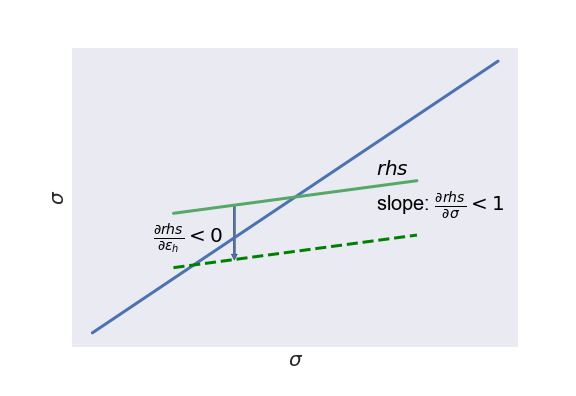
\includegraphics[width=.9\linewidth]{./fixedpoint.png}
\caption{\label{fig:fixedpoint}Solving equation \eqref{eq:37} for \(\sigma\).}
\end{figure}

We will show that \(\partial rhs/\partial \sigma \in \langle 0,1 \rangle\) and hence a change in a variable that shifts \(rhs\) up (down) will increase (decrease) \(\sigma\) in \eqref{eq:37}; see Figure \ref{fig:fixedpoint}. Hence, we want to show that
\begin{equation}
\label{eq:25}
\frac{\partial rhs}{\partial \sigma} = \frac{\Delta \sigma}{(\sigma+\Delta \sigma)^2} \frac{(1-\phi) \varepsilon_h c_h}{\phi \varepsilon_l + (1-\phi) \varepsilon_h -1} < 1
\end{equation}
while it is obvious that \(\partial rhs/\partial \sigma >0\). Equivalently
\begin{equation}
\label{eq:27}
\frac{\Delta \sigma}{\sigma + \Delta \sigma} \frac{c_h}{\Delta \sigma + \sigma}(1-\phi)\varepsilon_h < \phi \varepsilon_l + (1-\phi) \varepsilon_h -1
\end{equation}
Combining this with equation \eqref{eq:54} we find
\begin{equation}
\label{eq:30}
\frac{\Delta \sigma}{\sigma+\Delta \sigma}\frac{c_h}{\sigma+\Delta\sigma}(1-\phi)\varepsilon_h < \phi \frac{c_l}{\sigma}+(1-\phi)\varepsilon_h \frac{c_h}{\sigma+\Delta\sigma}
\end{equation}
which clearly holds because \(\Delta\sigma/(\Delta\sigma+\sigma) \leq 1\). Hence, we have found that \(\partial rhs/\partial \sigma < 1\).

To derive the effect of \(\varepsilon_h\) on \(\sigma\), we need to find \(\partial rhs/\partial \varepsilon_h\). It is routine to verify that
\begin{equation}
\label{eq:58}
\frac{\partial rhs}{\partial \varepsilon_h} =
(1-\phi) \frac{\phi \varepsilon_l (c_h \frac{\sigma}{\sigma+\Delta\sigma}-c_l)-c_h \frac{\sigma}{\sigma+\Delta\sigma}}{(\phi \varepsilon_l + (1-\phi)\varepsilon_h -1)^2} < 0
\end{equation}
To prove this inequality, first consider the case of \(\Delta \sigma=0\), i.e. we are back in the pooling contract. We know from equation \eqref{eq:26} and \(\lambda_l>0\) that \(\mu_h>0\). Equation \eqref{eq:29a} then implies the inequality in \eqref{eq:58}. Next consider \(\Delta \sigma > 0\). For \(\Delta \sigma\) big enough, the expression in \eqref{eq:58} is also negative. Finally, note that the sign of the derivative of the right hand side of \eqref{eq:58} with respect to \(\Delta \sigma\) does not vary with \(\Delta \sigma\) nor with \(\sigma\). That is, it cannot feature a maximum where the numerator of \eqref{eq:58} is positive. Hence, irrespective of the sign of this derivative, we see that \eqref{eq:58} is negative for all \(\Delta \sigma > 0\).

As \(\varepsilon_h\) increases, \(rhs\) shifts downwards in Figure \ref{fig:fixedpoint} and \(\sigma\) falls. Hence, we find that
\begin{equation}
\label{eq:45}
\frac{d\left(\frac{p_i-v_i}{v_i} \right)}{d \varepsilon_h} = - \frac{\phi}{1-\phi} \frac{\Delta \psi_i}{\psi_{ih}} \frac{\varepsilon_l c_l}{\sigma^2} \frac{d\sigma}{d\varepsilon_h} > 0
\end{equation}

To find the effect of \(\varepsilon_l\), we use equation \eqref{eq:26} for \(\lambda_l\) and hence we write
\begin{equation}
\label{eq:61}
\frac{p_i-v_i}{v_i} = \frac{\Delta\psi_i}{\psi_{ih}} \left(\varepsilon_h \left( 1-\frac{c_h}{\sigma+\Delta\sigma}\right)-1 \right)
\end{equation}
To find \(d\sigma/d\varepsilon_l\), we consider \(\partial rhs/\partial \varepsilon_l\). It is routine to verify that the sign of this derivative equals the sign of the following expression:
\begin{equation}
\label{eq:62}
(1-\phi) \varepsilon_h \left(c_l-c_h \frac{\sigma}{\sigma+\Delta\sigma} \right) - c_l
\end{equation}
This expression is negative, as can be seen as follows. We know from Lemma \ref{Linear_pricing_profit_margins} that \(\mu_l>\mu_h\) which can be written as
\begin{equation}
\label{eq:70}
1-\frac{c_l}{\sigma} > 1-\frac{c_h}{\sigma+\Delta\sigma}
\end{equation}
or equivalently
\begin{equation}
\label{eq:71}
\frac{c_l}{\sigma} < \frac{c_h}{\sigma+\Delta\sigma}
\end{equation}
from which it follows that \eqref{eq:62} is negative. Thus we find that \(d\sigma/d\varepsilon_l<0\).

Next, consider \(c_h\). We find that
\begin{equation}
\label{eq:57}
\frac{d\left(\frac{p_i-v_i}{v_i} \right)}{d c_h} = - \frac{\phi}{1-\phi} \frac{\Delta \psi_i}{\psi_{ih}} \frac{\varepsilon_l c_l}{\sigma^2} \frac{d\sigma}{d c_h}
\end{equation}
Since it is obvious that \(\partial rhs/\partial c_h >0\), we find that \(d\sigma/dc_h>0\) and hence supra profits fall with \(c_h\).

For \(c_l\), we define \(\tilde \sigma = \sigma/c_l\) and we write equation \eqref{eq:37} as
\begin{equation}
\label{eq:64}
\tilde \sigma = \frac{\phi \varepsilon_l +(1-\phi) \varepsilon_h c_h \frac{\tilde \sigma}{\tilde \sigma c_l + \Delta \sigma} }{\phi \varepsilon_l +(1-\phi) \varepsilon_h-1}
\end{equation}
It is clear that \(\partial rhs/\partial c_l <0\) and hence \(\partial \tilde \sigma /\partial c_l <0\). This implies that \(\partial (c_l/\sigma)\partial c_l > 0\) and therefore:
\begin{equation}
\label{eq:65}
\frac{d\left(\frac{p_i-v_i}{v_i} \right)}{dc_l} >0
\end{equation}

The effect of \(\zeta_i\) is obvious: since we assume that there are many treatments covered by insurance so that the effect of \(\zeta_i\) on \(\sigma\) is negligible, we have \(d(\Delta\psi_i/\psi_{ih})/d\zeta_i>0\). 
 \qed

\textbf{Proof of Corollary \ref{Targeting_profitable}}
We find the following derivative
\begin{equation}
\label{eq:66}
\frac{d \pi_i}{d \zeta_i} = (1-\phi) \frac{d \psi_{ih}}{d\zeta_i} v_i+\phi \frac{d\Delta\psi_i}{d\zeta_i}v_i (1-\varepsilon_h(1-\frac{c_l}{\sigma})) > 0
\end{equation}
for \(\phi\) close enough to 1 because \(d\psi_{ih}/d\zeta_{i}<0\) and \(d\Delta\psi_i/d\zeta_i>0\). 
 \qed

\subsection{Bounded rationality}
\label{sec:org54662df}

\begin{proposition}
\label{propBounded}
For \(\delta_{il} > 0\) but small, charging \(p_i>v_i\) is optimal and the insurance contract is sold to both the \(h\) and \(l\) type.
For high \(\delta_{il}>0\), a further increase in \(\delta_{il}\) reduces \(p_{il}\).
\end{proposition}

\textbf{Proof of proposition \ref{propBounded}}
It is routine to verify that profit function \(\Pi^{\iota}\) in equation \eqref{eq:15} can now be written as:
\begin{equation}
\label{eq:15b}
\begin{split}
\Pi^{\iota} &= \phi q^{\iota}(u_l^{\iota},u_l^{-\iota},\theta_l) (\sum_{i \in P} \alpha_i x_{il}^{\iota}[\psi_{il}(v_i-p_i)+v_i \delta_{il}] + \sum_{j \in O} \psi_{jl} x_{jl}^{\iota} v_j - u_l^{\iota}) \\
    &+ (1-\phi) q^{\iota}(u_h^{\iota},u_h^{-\iota},\theta_h) (\sum_{i \in P} \alpha_i \psi_{ih} x_{ih}^{\iota} (v_i-p_i) + \sum_{j \in O} \psi_{jh} x_{jh}^{\iota} v_j - u_h^{\iota}) \\
    &+ \lambda_l (u_l^{\iota} - u_h^{\iota} + \sum_{i \in P} \alpha_i x_{ih}^{\iota} v_i (\Delta\psi_{i}-\delta_{il}) + \sum_{j \in O} x_{jh}^{\iota} v_j \Delta\psi_{j})
\end{split}
\end{equation}
where expressions with \(\delta_{il}\) are added to the first and last line and we focus on the case with \(\lambda_l>\lambda_h =0\).

The first order conditions for most variables are the same as above, with two exceptions. First, the first order condition for \(x_{il}^{\iota}\) shows that \(x_{il}=1\) if and only if
\begin{equation}
\label{eq:44}
(v_i-p_i)\psi_{il}+v_i \delta_{il} \geq 0
\end{equation}
or equivalently
\begin{equation}
\label{eq:49}
p_i \leq v_i \left(1+\frac{\delta_{il}}{\psi_{il}} \right)
\end{equation}
Second, the first order condition for \(x_{ih}^{\iota}\) implies that \(x_{ih}=1\) if and only if
\begin{equation}
\label{eq:72}
p_i \leq v_i \left(1+\lambda_l \frac{\Delta \psi_i -\delta_{il}}{(1-\phi)\frac{1}{n} \psi_{ih}} \right)
\end{equation}
in symmetric equilibrium with \(q^{\iota}(.)=1/n\).

Hence, we can have a pooling contract with \(x_{il}=x_{ih}=1\) for \(p_i>v_i\) as long as both \eqref{eq:49} and \eqref{eq:72} hold. Therefore, for \(\delta_{il} > 0\) but small, we extend the range of parameters for which it is optimal for research lab \(i\) to induce a pooling contract instead of charging \(p_i\) so high that treatment \(i\) is dropped from \(l\) type's contract. As \(\delta_i\) increases, so does \(p_i\). However, for high \(\delta_i\), \(l\) types over-estimate the probability \(\psi_{il}\) to such an extent that treatment \(i\) is no longer useful in separating the types. If \(l\) types believe that their probability of needing \(i\) is the same as for \(h\) types, we have \(\delta_{il} = \Delta \psi_i\) and equation \eqref{eq:72} implies \(p_i \leq v_i\).

 \qed
\end{document}